% Options for packages loaded elsewhere
\PassOptionsToPackage{unicode}{hyperref}
\PassOptionsToPackage{hyphens}{url}
%
\documentclass[
]{article}
\usepackage{amsmath,amssymb}
\usepackage{iftex}
\ifPDFTeX
  \usepackage[T1]{fontenc}
  \usepackage[utf8]{inputenc}
  \usepackage{textcomp} % provide euro and other symbols
\else % if luatex or xetex
  \usepackage{unicode-math} % this also loads fontspec
  \defaultfontfeatures{Scale=MatchLowercase}
  \defaultfontfeatures[\rmfamily]{Ligatures=TeX,Scale=1}
\fi
\usepackage{lmodern}
\ifPDFTeX\else
  % xetex/luatex font selection
\fi
% Use upquote if available, for straight quotes in verbatim environments
\IfFileExists{upquote.sty}{\usepackage{upquote}}{}
\IfFileExists{microtype.sty}{% use microtype if available
  \usepackage[]{microtype}
  \UseMicrotypeSet[protrusion]{basicmath} % disable protrusion for tt fonts
}{}
\makeatletter
\@ifundefined{KOMAClassName}{% if non-KOMA class
  \IfFileExists{parskip.sty}{%
    \usepackage{parskip}
  }{% else
    \setlength{\parindent}{0pt}
    \setlength{\parskip}{6pt plus 2pt minus 1pt}}
}{% if KOMA class
  \KOMAoptions{parskip=half}}
\makeatother
\usepackage{xcolor}
\usepackage[margin=1in]{geometry}
\usepackage{color}
\usepackage{fancyvrb}
\newcommand{\VerbBar}{|}
\newcommand{\VERB}{\Verb[commandchars=\\\{\}]}
\DefineVerbatimEnvironment{Highlighting}{Verbatim}{commandchars=\\\{\}}
% Add ',fontsize=\small' for more characters per line
\usepackage{framed}
\definecolor{shadecolor}{RGB}{248,248,248}
\newenvironment{Shaded}{\begin{snugshade}}{\end{snugshade}}
\newcommand{\AlertTok}[1]{\textcolor[rgb]{0.94,0.16,0.16}{#1}}
\newcommand{\AnnotationTok}[1]{\textcolor[rgb]{0.56,0.35,0.01}{\textbf{\textit{#1}}}}
\newcommand{\AttributeTok}[1]{\textcolor[rgb]{0.13,0.29,0.53}{#1}}
\newcommand{\BaseNTok}[1]{\textcolor[rgb]{0.00,0.00,0.81}{#1}}
\newcommand{\BuiltInTok}[1]{#1}
\newcommand{\CharTok}[1]{\textcolor[rgb]{0.31,0.60,0.02}{#1}}
\newcommand{\CommentTok}[1]{\textcolor[rgb]{0.56,0.35,0.01}{\textit{#1}}}
\newcommand{\CommentVarTok}[1]{\textcolor[rgb]{0.56,0.35,0.01}{\textbf{\textit{#1}}}}
\newcommand{\ConstantTok}[1]{\textcolor[rgb]{0.56,0.35,0.01}{#1}}
\newcommand{\ControlFlowTok}[1]{\textcolor[rgb]{0.13,0.29,0.53}{\textbf{#1}}}
\newcommand{\DataTypeTok}[1]{\textcolor[rgb]{0.13,0.29,0.53}{#1}}
\newcommand{\DecValTok}[1]{\textcolor[rgb]{0.00,0.00,0.81}{#1}}
\newcommand{\DocumentationTok}[1]{\textcolor[rgb]{0.56,0.35,0.01}{\textbf{\textit{#1}}}}
\newcommand{\ErrorTok}[1]{\textcolor[rgb]{0.64,0.00,0.00}{\textbf{#1}}}
\newcommand{\ExtensionTok}[1]{#1}
\newcommand{\FloatTok}[1]{\textcolor[rgb]{0.00,0.00,0.81}{#1}}
\newcommand{\FunctionTok}[1]{\textcolor[rgb]{0.13,0.29,0.53}{\textbf{#1}}}
\newcommand{\ImportTok}[1]{#1}
\newcommand{\InformationTok}[1]{\textcolor[rgb]{0.56,0.35,0.01}{\textbf{\textit{#1}}}}
\newcommand{\KeywordTok}[1]{\textcolor[rgb]{0.13,0.29,0.53}{\textbf{#1}}}
\newcommand{\NormalTok}[1]{#1}
\newcommand{\OperatorTok}[1]{\textcolor[rgb]{0.81,0.36,0.00}{\textbf{#1}}}
\newcommand{\OtherTok}[1]{\textcolor[rgb]{0.56,0.35,0.01}{#1}}
\newcommand{\PreprocessorTok}[1]{\textcolor[rgb]{0.56,0.35,0.01}{\textit{#1}}}
\newcommand{\RegionMarkerTok}[1]{#1}
\newcommand{\SpecialCharTok}[1]{\textcolor[rgb]{0.81,0.36,0.00}{\textbf{#1}}}
\newcommand{\SpecialStringTok}[1]{\textcolor[rgb]{0.31,0.60,0.02}{#1}}
\newcommand{\StringTok}[1]{\textcolor[rgb]{0.31,0.60,0.02}{#1}}
\newcommand{\VariableTok}[1]{\textcolor[rgb]{0.00,0.00,0.00}{#1}}
\newcommand{\VerbatimStringTok}[1]{\textcolor[rgb]{0.31,0.60,0.02}{#1}}
\newcommand{\WarningTok}[1]{\textcolor[rgb]{0.56,0.35,0.01}{\textbf{\textit{#1}}}}
\usepackage{graphicx}
\makeatletter
\def\maxwidth{\ifdim\Gin@nat@width>\linewidth\linewidth\else\Gin@nat@width\fi}
\def\maxheight{\ifdim\Gin@nat@height>\textheight\textheight\else\Gin@nat@height\fi}
\makeatother
% Scale images if necessary, so that they will not overflow the page
% margins by default, and it is still possible to overwrite the defaults
% using explicit options in \includegraphics[width, height, ...]{}
\setkeys{Gin}{width=\maxwidth,height=\maxheight,keepaspectratio}
% Set default figure placement to htbp
\makeatletter
\def\fps@figure{htbp}
\makeatother
\setlength{\emergencystretch}{3em} % prevent overfull lines
\providecommand{\tightlist}{%
  \setlength{\itemsep}{0pt}\setlength{\parskip}{0pt}}
\setcounter{secnumdepth}{-\maxdimen} % remove section numbering
\usepackage{booktabs}
\usepackage{float}
\floatplacement{figure}{H}
\usepackage{booktabs}
\usepackage{longtable}
\usepackage{array}
\usepackage{multirow}
\usepackage{wrapfig}
\usepackage{float}
\usepackage{colortbl}
\usepackage{pdflscape}
\usepackage{tabu}
\usepackage{threeparttable}
\usepackage{threeparttablex}
\usepackage[normalem]{ulem}
\usepackage{makecell}
\usepackage{xcolor}
\ifLuaTeX
  \usepackage{selnolig}  % disable illegal ligatures
\fi
\usepackage{bookmark}
\IfFileExists{xurl.sty}{\usepackage{xurl}}{} % add URL line breaks if available
\urlstyle{same}
\hypersetup{
  pdftitle={California Road Construction Safety Analysis: A Spatial Econometric Approach},
  pdfauthor={Moritz Peist; Noemi Lucchi; Simon Vellin},
  hidelinks,
  pdfcreator={LaTeX via pandoc}}

\title{California Road Construction Safety Analysis: A Spatial
Econometric Approach}
\author{Moritz Peist \and Noemi Lucchi \and Simon Vellin}
\date{März 26, 2025}

\begin{document}
\maketitle

{
\setcounter{tocdepth}{3}
\tableofcontents
}
\subsection{Abstract}\label{abstract}

This study examines the causal relationship between road construction
activities and traffic accident rates in California using
high-resolution spatial data from 2021. Implementing a
difference-in-differences framework with spatial controls, we analyze
how construction zones affect accident frequency and severity. Our
findings indicate a significant positive relationship between active
construction and accident occurrence, with heterogeneous effects across
urban and rural environments. Specifically, we observe that the effect
of construction on accident rates is substantially larger in urban
areas. Spatial spillover analysis reveals that accident impacts extend
beyond immediate construction zones, with particularly strong effects in
areas 500-1000m from construction sites. This research provides
evidence-based insights for transportation safety planning and targeted
mitigation strategies.

\subsection{1. Introduction}\label{introduction}

Road construction is a necessary yet potentially disruptive component of
transportation infrastructure maintenance and development. While
essential for long-term safety improvements, construction activities
create temporary changes in traffic patterns, road conditions, and
driver behavior that may increase accident risk. Understanding the
causal relationship between construction activities and traffic safety
has important implications for construction scheduling, resource
allocation, traffic management strategies, and policy development.

Despite the importance of this relationship, rigorous causal evidence on
how road construction affects traffic accidents remains limited,
particularly with respect to potential heterogeneity between urban and
rural environments. This study addresses this gap by leveraging
comprehensive spatial data on road construction activities and traffic
accidents in California during 2021 to answer the following research
questions:

\begin{enumerate}
\def\labelenumi{\arabic{enumi}.}
\tightlist
\item
  How does road construction causally impact traffic accident rates?
\item
  Do these effects systematically differ between urban and rural
  environments?
\item
  Are there spatial spillover effects beyond the immediate construction
  zones?
\end{enumerate}

The findings of this research have direct implications for
transportation safety planning, particularly regarding how resources
should be allocated for traffic management during construction
activities across different environments.

\subsection{2. Data and Methods}\label{data-and-methods}

\subsubsection{2.1 Data Sources}\label{data-sources}

This study integrates multiple large-scale datasets to create a
comprehensive spatial-temporal framework for analysis:

\textbf{Primary Datasets:} 1. \textbf{US Road Construction and Closures
Dataset (2021)} - Contains detailed records of construction activities
in California with coordinates, start/end times, and affected distances
2. \textbf{US Traffic Accidents Dataset (2021)} - Comprehensive accident
records with precise locations, timestamps, and severity measures 3.
\textbf{Caltrans State Highway Network} - Annual Average Daily Traffic
(AADT) data for normalizing accident rates by traffic volume 4.
\textbf{US Census Bureau Urban Areas} - Official urban/rural
classifications for spatial heterogeneity analysis

\subsubsection{2.2 Data Processing and
Preparation}\label{data-processing-and-preparation}

We focused our analysis on California road construction and accidents
from 2021, creating a spatial-temporal framework that allows us to
examine the causal relationship between construction activities and
accidents.

\begin{Shaded}
\begin{Highlighting}[]
\CommentTok{\# Load Caltrans State Highway Network}
\NormalTok{aadt }\OtherTok{\textless{}{-}} \FunctionTok{st\_read}\NormalTok{(}\StringTok{"data/Traffic\_Volumes\_AADT/Traffic\_Volumes\_AADT.shp"}\NormalTok{)}

\CommentTok{\# Load and filter accidents data}
\NormalTok{df.acc }\OtherTok{\textless{}{-}} \FunctionTok{fread}\NormalTok{(}\StringTok{"data/us\_accidents/US\_accidents\_March23.csv"}\NormalTok{)[}
  \CommentTok{\# Filter date range of 2021}
\NormalTok{  lubridate}\SpecialCharTok{::}\FunctionTok{year}\NormalTok{(}\FunctionTok{as.Date}\NormalTok{(Start\_Time)) }\SpecialCharTok{==} \DecValTok{2021} \SpecialCharTok{\&} 
  \CommentTok{\# And California}
\NormalTok{  State }\SpecialCharTok{==} \StringTok{"CA"}
\NormalTok{][, }\StringTok{\textasciigrave{}}\AttributeTok{:=}\StringTok{\textasciigrave{}}\NormalTok{(}
  \CommentTok{\# Add year, quarter, month columns}
  \AttributeTok{year =}\NormalTok{ data.table}\SpecialCharTok{::}\FunctionTok{year}\NormalTok{(Start\_Time),}
  \AttributeTok{quarter =}\NormalTok{ data.table}\SpecialCharTok{::}\FunctionTok{quarter}\NormalTok{(Start\_Time),}
  \AttributeTok{month =}\NormalTok{ data.table}\SpecialCharTok{::}\FunctionTok{month}\NormalTok{(Start\_Time),}
  \CommentTok{\# Calculate duration}
  \AttributeTok{duration =} \FunctionTok{as.numeric}\NormalTok{(}\FunctionTok{difftime}\NormalTok{(End\_Time, Start\_Time, }\AttributeTok{units =} \StringTok{"days"}\NormalTok{))}
\NormalTok{)] }\SpecialCharTok{\%\textgreater{}\%} 
  \FunctionTok{as\_tibble}\NormalTok{()}

\CommentTok{\# Load and filter construction data}
\NormalTok{df.const }\OtherTok{\textless{}{-}} \FunctionTok{fread}\NormalTok{(}\StringTok{"data/us\_constructions/US\_constructions\_Dec21.csv"}\NormalTok{)[}
  \CommentTok{\# Filter date range of 2021}
\NormalTok{  lubridate}\SpecialCharTok{::}\FunctionTok{year}\NormalTok{(}\FunctionTok{as.Date}\NormalTok{(Start\_Time)) }\SpecialCharTok{==} \DecValTok{2021} \SpecialCharTok{\&} 
  \CommentTok{\# And California}
\NormalTok{  State }\SpecialCharTok{==} \StringTok{"CA"}
\NormalTok{][, }\StringTok{\textasciigrave{}}\AttributeTok{:=}\StringTok{\textasciigrave{}}\NormalTok{(}
  \CommentTok{\# Add year, quarter, month columns}
  \AttributeTok{year =} \FunctionTok{year}\NormalTok{(Start\_Time),}
  \AttributeTok{quarter =} \FunctionTok{quarter}\NormalTok{(Start\_Time),}
  \AttributeTok{month =} \FunctionTok{month}\NormalTok{(Start\_Time),}
  \CommentTok{\# Calculate duration}
  \AttributeTok{duration =} \FunctionTok{as.numeric}\NormalTok{(}\FunctionTok{difftime}\NormalTok{(End\_Time, Start\_Time, }\AttributeTok{units =} \StringTok{"days"}\NormalTok{))}
\NormalTok{)][}
\NormalTok{  duration }\SpecialCharTok{\textgreater{}} \DecValTok{1}  \CommentTok{\# Filter out constructions lasting less than a day}
\NormalTok{] }\SpecialCharTok{\%\textgreater{}\%} 
  \FunctionTok{as\_tibble}\NormalTok{()}
\end{Highlighting}
\end{Shaded}

\begin{Shaded}
\begin{Highlighting}[]
\CommentTok{\# Display data summary (using pre{-}computed values for reproducibility)}
\NormalTok{accidents\_count }\OtherTok{\textless{}{-}} \DecValTok{341876}
\NormalTok{construction\_count }\OtherTok{\textless{}{-}} \DecValTok{33513}
\NormalTok{aadt\_count }\OtherTok{\textless{}{-}} \DecValTok{13874}

\FunctionTok{cat}\NormalTok{(}\StringTok{"Summary of datasets:}\SpecialCharTok{\textbackslash{}n}\StringTok{"}\NormalTok{)}
\end{Highlighting}
\end{Shaded}

\begin{verbatim}
## Summary of datasets:
\end{verbatim}

\begin{Shaded}
\begin{Highlighting}[]
\FunctionTok{cat}\NormalTok{(}\StringTok{"{-} Accidents dataset:"}\NormalTok{, accidents\_count, }\StringTok{"records}\SpecialCharTok{\textbackslash{}n}\StringTok{"}\NormalTok{)}
\end{Highlighting}
\end{Shaded}

\begin{verbatim}
## - Accidents dataset: 341876 records
\end{verbatim}

\begin{Shaded}
\begin{Highlighting}[]
\FunctionTok{cat}\NormalTok{(}\StringTok{"{-} Construction dataset:"}\NormalTok{, construction\_count, }\StringTok{"records}\SpecialCharTok{\textbackslash{}n}\StringTok{"}\NormalTok{)}
\end{Highlighting}
\end{Shaded}

\begin{verbatim}
## - Construction dataset: 33513 records
\end{verbatim}

\begin{Shaded}
\begin{Highlighting}[]
\FunctionTok{cat}\NormalTok{(}\StringTok{"{-} AADT dataset:"}\NormalTok{, aadt\_count, }\StringTok{"records}\SpecialCharTok{\textbackslash{}n}\StringTok{"}\NormalTok{)}
\end{Highlighting}
\end{Shaded}

\begin{verbatim}
## - AADT dataset: 13874 records
\end{verbatim}

The data preparation revealed 341,876 accident records and 33,513
construction events across California in 2021. The temporal distribution
of both accidents and construction projects showed seasonal patterns,
with construction activity peaking in the spring months and accidents
showing higher frequency in winter and fall.

\begin{Shaded}
\begin{Highlighting}[]
\CommentTok{\# Temporal patterns visualization}
\NormalTok{acc\_monthly }\OtherTok{\textless{}{-}}\NormalTok{ df.acc }\SpecialCharTok{\%\textgreater{}\%}
  \FunctionTok{mutate}\NormalTok{(}\AttributeTok{month =} \FunctionTok{floor\_date}\NormalTok{(}\FunctionTok{as.Date}\NormalTok{(Start\_Time), }\StringTok{"month"}\NormalTok{)) }\SpecialCharTok{\%\textgreater{}\%}
  \FunctionTok{count}\NormalTok{(month)}

\NormalTok{const\_monthly }\OtherTok{\textless{}{-}}\NormalTok{ df.const }\SpecialCharTok{\%\textgreater{}\%}
  \FunctionTok{mutate}\NormalTok{(}\AttributeTok{month =} \FunctionTok{floor\_date}\NormalTok{(}\FunctionTok{as.Date}\NormalTok{(Start\_Time), }\StringTok{"month"}\NormalTok{)) }\SpecialCharTok{\%\textgreater{}\%}
  \FunctionTok{count}\NormalTok{(month)}

\CommentTok{\# Plot monthly patterns}
\NormalTok{p1 }\OtherTok{\textless{}{-}} \FunctionTok{ggplot}\NormalTok{(acc\_monthly, }\FunctionTok{aes}\NormalTok{(}\AttributeTok{x =}\NormalTok{ month, }\AttributeTok{y =}\NormalTok{ n)) }\SpecialCharTok{+}
  \FunctionTok{geom\_line}\NormalTok{(}\AttributeTok{color =} \StringTok{"blue"}\NormalTok{) }\SpecialCharTok{+}
  \FunctionTok{geom\_point}\NormalTok{(}\AttributeTok{color =} \StringTok{"blue"}\NormalTok{) }\SpecialCharTok{+}
  \FunctionTok{labs}\NormalTok{(}\AttributeTok{title =} \StringTok{"Monthly Accidents in California (2021)"}\NormalTok{,}
       \AttributeTok{x =} \StringTok{"Month"}\NormalTok{, }\AttributeTok{y =} \StringTok{"Count"}\NormalTok{) }\SpecialCharTok{+}
  \FunctionTok{theme\_minimal}\NormalTok{()}

\NormalTok{p2 }\OtherTok{\textless{}{-}} \FunctionTok{ggplot}\NormalTok{(const\_monthly, }\FunctionTok{aes}\NormalTok{(}\AttributeTok{x =}\NormalTok{ month, }\AttributeTok{y =}\NormalTok{ n)) }\SpecialCharTok{+}
  \FunctionTok{geom\_line}\NormalTok{(}\AttributeTok{color =} \StringTok{"red"}\NormalTok{) }\SpecialCharTok{+}
  \FunctionTok{geom\_point}\NormalTok{(}\AttributeTok{color =} \StringTok{"red"}\NormalTok{) }\SpecialCharTok{+}
  \FunctionTok{labs}\NormalTok{(}\AttributeTok{title =} \StringTok{"New Construction Projects in California (2021)"}\NormalTok{,}
       \AttributeTok{x =} \StringTok{"Month"}\NormalTok{, }\AttributeTok{y =} \StringTok{"Count"}\NormalTok{) }\SpecialCharTok{+}
  \FunctionTok{theme\_minimal}\NormalTok{()}

\NormalTok{p1 }\SpecialCharTok{+}\NormalTok{ p2}
\end{Highlighting}
\end{Shaded}

\begin{Shaded}
\begin{Highlighting}[]
\CommentTok{\# Check construction durations}
\NormalTok{df.const }\SpecialCharTok{\%\textgreater{}\%}
  \FunctionTok{ggplot}\NormalTok{(}\FunctionTok{aes}\NormalTok{(}\AttributeTok{x =}\NormalTok{ duration)) }\SpecialCharTok{+}
  \FunctionTok{geom\_histogram}\NormalTok{(}\AttributeTok{bins =} \DecValTok{30}\NormalTok{, }\AttributeTok{fill =} \StringTok{"orange"}\NormalTok{) }\SpecialCharTok{+}
  \FunctionTok{labs}\NormalTok{(}\AttributeTok{title =} \StringTok{"Distribution of Construction Duration"}\NormalTok{,}
       \AttributeTok{x =} \StringTok{"Duration (days)"}\NormalTok{, }\AttributeTok{y =} \StringTok{"Count"}\NormalTok{) }\SpecialCharTok{+}
  \FunctionTok{theme\_minimal}\NormalTok{()}
\end{Highlighting}
\end{Shaded}

\subsubsection{2.3 Methodology}\label{methodology}

Our analysis employs a difference-in-differences (DiD) framework
augmented with spatial controls to identify the causal impact of
construction activities on traffic accidents. This approach allows us to
address potential endogeneity concerns by controlling for time-invariant
location characteristics and time-specific effects.

\paragraph{2.3.1 Spatial Processing}\label{spatial-processing}

To establish the spatial relationship between accidents and construction
activities, we converted both accident and construction datasets to
spatial objects and created 500-meter buffer zones around construction
locations. These buffer zones served as our treatment areas.

\begin{Shaded}
\begin{Highlighting}[]
\CommentTok{\# Create spatial objects}
\ControlFlowTok{if}\NormalTok{ (}\SpecialCharTok{!}\FunctionTok{inherits}\NormalTok{(df.acc, }\StringTok{"sf"}\NormalTok{)) \{}
\NormalTok{  df.acc.sf }\OtherTok{\textless{}{-}}\NormalTok{ df.acc }\SpecialCharTok{\%\textgreater{}\%}
    \FunctionTok{filter}\NormalTok{(}\SpecialCharTok{!}\FunctionTok{is.na}\NormalTok{(Start\_Lat) }\SpecialCharTok{\&} \SpecialCharTok{!}\FunctionTok{is.na}\NormalTok{(Start\_Lng)) }\SpecialCharTok{\%\textgreater{}\%}
    \FunctionTok{st\_as\_sf}\NormalTok{(}\AttributeTok{coords =} \FunctionTok{c}\NormalTok{(}\StringTok{"Start\_Lng"}\NormalTok{, }\StringTok{"Start\_Lat"}\NormalTok{), }\AttributeTok{crs =} \DecValTok{4326}\NormalTok{) }\SpecialCharTok{\%\textgreater{}\%}
    \FunctionTok{st\_transform}\NormalTok{(}\AttributeTok{crs =} \DecValTok{3310}\NormalTok{)  }\CommentTok{\# CA Albers for accurate distance}
\NormalTok{\} }\ControlFlowTok{else}\NormalTok{ \{}
\NormalTok{  df.acc.sf }\OtherTok{\textless{}{-}}\NormalTok{ df.acc}
\NormalTok{\}}

\ControlFlowTok{if}\NormalTok{ (}\SpecialCharTok{!}\FunctionTok{inherits}\NormalTok{(df.const, }\StringTok{"sf"}\NormalTok{)) \{}
\NormalTok{  df.const.sf }\OtherTok{\textless{}{-}}\NormalTok{ df.const }\SpecialCharTok{\%\textgreater{}\%}
    \FunctionTok{filter}\NormalTok{(}\SpecialCharTok{!}\FunctionTok{is.na}\NormalTok{(Start\_Lat) }\SpecialCharTok{\&} \SpecialCharTok{!}\FunctionTok{is.na}\NormalTok{(Start\_Lng)) }\SpecialCharTok{\%\textgreater{}\%}
    \FunctionTok{st\_as\_sf}\NormalTok{(}\AttributeTok{coords =} \FunctionTok{c}\NormalTok{(}\StringTok{"Start\_Lng"}\NormalTok{, }\StringTok{"Start\_Lat"}\NormalTok{), }\AttributeTok{crs =} \DecValTok{4326}\NormalTok{) }\SpecialCharTok{\%\textgreater{}\%}
    \FunctionTok{st\_transform}\NormalTok{(}\AttributeTok{crs =} \DecValTok{3310}\NormalTok{)}
\NormalTok{\} }\ControlFlowTok{else}\NormalTok{ \{}
\NormalTok{  df.const.sf }\OtherTok{\textless{}{-}}\NormalTok{ df.const}
\NormalTok{\}}

\CommentTok{\# Create construction buffers (500m)}
\NormalTok{const\_buffers }\OtherTok{\textless{}{-}}\NormalTok{ df.const.sf }\SpecialCharTok{\%\textgreater{}\%}
  \FunctionTok{st\_buffer}\NormalTok{(}\AttributeTok{dist =} \DecValTok{500}\NormalTok{)  }\CommentTok{\# 500m buffer}

\CommentTok{\# Add buffer metadata}
\NormalTok{const\_buffers }\OtherTok{\textless{}{-}}\NormalTok{ const\_buffers }\SpecialCharTok{\%\textgreater{}\%}
  \FunctionTok{mutate}\NormalTok{(}
    \AttributeTok{buffer\_id =} \FunctionTok{paste0}\NormalTok{(}\StringTok{"c"}\NormalTok{, }\FunctionTok{row\_number}\NormalTok{()),}
    \AttributeTok{start\_date =} \FunctionTok{as.Date}\NormalTok{(Start\_Time),}
    \AttributeTok{end\_date =} \FunctionTok{as.Date}\NormalTok{(End\_Time),}
    \AttributeTok{construction\_duration =} \FunctionTok{as.numeric}\NormalTok{(}\FunctionTok{difftime}\NormalTok{(end\_date, start\_date, }\AttributeTok{units =} \StringTok{"days"}\NormalTok{))}
\NormalTok{  )}
\end{Highlighting}
\end{Shaded}

\paragraph{2.3.2 Urban-Rural
Classification}\label{urban-rural-classification}

We classified construction sites as urban or rural based on their
intersection with US Census Bureau urban areas. This classification is
crucial for our heterogeneity analysis.

\begin{Shaded}
\begin{Highlighting}[]
\CommentTok{\# Download urban areas for California}
\NormalTok{ca\_urban\_areas }\OtherTok{\textless{}{-}}\NormalTok{ tigris}\SpecialCharTok{::}\FunctionTok{urban\_areas}\NormalTok{(}\AttributeTok{cb =} \ConstantTok{TRUE}\NormalTok{, }\AttributeTok{year =} \DecValTok{2019}\NormalTok{) }\SpecialCharTok{\%\textgreater{}\%}
  \FunctionTok{st\_transform}\NormalTok{(}\FunctionTok{st\_crs}\NormalTok{(const\_buffers)) }\SpecialCharTok{\%\textgreater{}\%}
  \FunctionTok{filter}\NormalTok{(}\FunctionTok{grepl}\NormalTok{(}\StringTok{", CA$"}\NormalTok{, NAME10))}

\CommentTok{\# Classify construction sites as urban or rural}
\NormalTok{const\_urban }\OtherTok{\textless{}{-}} \FunctionTok{st\_join}\NormalTok{(}
\NormalTok{  const\_buffers,}
\NormalTok{  ca\_urban\_areas }\SpecialCharTok{\%\textgreater{}\%} \FunctionTok{select}\NormalTok{(}\AttributeTok{urban\_name =}\NormalTok{ NAME10),}
  \AttributeTok{join =}\NormalTok{ st\_intersects}
\NormalTok{)}

\NormalTok{const\_urban }\OtherTok{\textless{}{-}}\NormalTok{ const\_urban }\SpecialCharTok{\%\textgreater{}\%}
  \FunctionTok{mutate}\NormalTok{(}\AttributeTok{is\_urban =} \SpecialCharTok{!}\FunctionTok{is.na}\NormalTok{(urban\_name))}

\CommentTok{\# Visualize urban/rural distribution}
\NormalTok{urban\_rural\_counts }\OtherTok{\textless{}{-}}\NormalTok{ const\_urban }\SpecialCharTok{\%\textgreater{}\%}
  \FunctionTok{st\_drop\_geometry}\NormalTok{() }\SpecialCharTok{\%\textgreater{}\%}
  \FunctionTok{count}\NormalTok{(is\_urban) }\SpecialCharTok{\%\textgreater{}\%}
  \FunctionTok{mutate}\NormalTok{(}\AttributeTok{percentage =}\NormalTok{ n }\SpecialCharTok{/} \FunctionTok{sum}\NormalTok{(n) }\SpecialCharTok{*} \DecValTok{100}\NormalTok{)}
\end{Highlighting}
\end{Shaded}

\begin{Shaded}
\begin{Highlighting}[]
\CommentTok{\# Urban{-}rural distribution (using pre{-}computed values)}
\NormalTok{urban\_rural\_df }\OtherTok{\textless{}{-}} \FunctionTok{data.frame}\NormalTok{(}
  \AttributeTok{is\_urban =} \FunctionTok{c}\NormalTok{(}\ConstantTok{FALSE}\NormalTok{, }\ConstantTok{TRUE}\NormalTok{),}
  \AttributeTok{n =} \FunctionTok{c}\NormalTok{(}\DecValTok{9803}\NormalTok{, }\DecValTok{23795}\NormalTok{),}
  \AttributeTok{percentage =} \FunctionTok{c}\NormalTok{(}\FloatTok{29.2}\NormalTok{, }\FloatTok{70.8}\NormalTok{)}
\NormalTok{)}

\NormalTok{kableExtra}\SpecialCharTok{::}\FunctionTok{kable}\NormalTok{(urban\_rural\_df, }
                 \AttributeTok{col.names =} \FunctionTok{c}\NormalTok{(}\StringTok{"Urban Area"}\NormalTok{, }\StringTok{"Count"}\NormalTok{, }\StringTok{"Percentage (\%)"}\NormalTok{),}
                 \AttributeTok{caption =} \StringTok{"Distribution of Construction Sites by Urban/Rural Classification"}\NormalTok{,}
                 \AttributeTok{booktabs =} \ConstantTok{TRUE}\NormalTok{,}
                 \AttributeTok{digits =} \DecValTok{1}\NormalTok{) }\SpecialCharTok{\%\textgreater{}\%}
\NormalTok{  kableExtra}\SpecialCharTok{::}\FunctionTok{kable\_styling}\NormalTok{(}\AttributeTok{latex\_options =} \FunctionTok{c}\NormalTok{(}\StringTok{"striped"}\NormalTok{, }\StringTok{"hold\_position"}\NormalTok{),}
                           \AttributeTok{full\_width =} \ConstantTok{FALSE}\NormalTok{) }\SpecialCharTok{\%\textgreater{}\%}
\NormalTok{  kableExtra}\SpecialCharTok{::}\FunctionTok{row\_spec}\NormalTok{(}\DecValTok{0}\NormalTok{, }\AttributeTok{bold =} \ConstantTok{TRUE}\NormalTok{) }\SpecialCharTok{\%\textgreater{}\%}
\NormalTok{  kableExtra}\SpecialCharTok{::}\FunctionTok{row\_spec}\NormalTok{(}\DecValTok{1}\SpecialCharTok{:}\DecValTok{2}\NormalTok{, }\AttributeTok{background =} \FunctionTok{c}\NormalTok{(}\StringTok{"\#f5f5f5"}\NormalTok{, }\StringTok{"\#e8e8e8"}\NormalTok{))}
\end{Highlighting}
\end{Shaded}

\begin{longtable}[t]{lrr}
\caption{\label{tab:urban_rural_table}Distribution of Construction Sites by Urban/Rural Classification}\\
\toprule
\textbf{Urban Area} & \textbf{Count} & \textbf{Percentage (\%)}\\
\midrule
\cellcolor[HTML]{f5f5f5}{\cellcolor{gray!10}{FALSE}} & \cellcolor[HTML]{e8e8e8}{\cellcolor{gray!10}{9803}} & \cellcolor[HTML]{f5f5f5}{\cellcolor{gray!10}{29.2}}\\
\cellcolor[HTML]{f5f5f5}{TRUE} & \cellcolor[HTML]{e8e8e8}{23795} & \cellcolor[HTML]{f5f5f5}{70.8}\\
\bottomrule
\end{longtable}

Our analysis revealed that approximately 70.8\% of construction zones
were located in urban areas, with the remaining 29.2\% in rural
environments.

\paragraph{2.3.3 Panel Dataset
Construction}\label{panel-dataset-construction}

We created a panel dataset that tracks accidents in each buffer zone
over time, with indicators for pre-construction, during-construction,
and post-construction periods. This approach allows us to implement the
difference-in-differences design.

\begin{Shaded}
\begin{Highlighting}[]
\CommentTok{\# Join accidents to construction buffers}
\NormalTok{accidents\_in\_buffers }\OtherTok{\textless{}{-}} \FunctionTok{st\_join}\NormalTok{(}
\NormalTok{  df.acc.sf }\SpecialCharTok{\%\textgreater{}\%} 
    \FunctionTok{select}\NormalTok{(}\AttributeTok{accident\_id =}\NormalTok{ ID, }\AttributeTok{accident\_date =}\NormalTok{ Start\_Time, Severity),}
\NormalTok{  const\_urban }\SpecialCharTok{\%\textgreater{}\%} 
    \FunctionTok{select}\NormalTok{(buffer\_id, }\AttributeTok{construction\_id =}\NormalTok{ ID, start\_date, end\_date, is\_urban),}
  \AttributeTok{join =}\NormalTok{ st\_intersects}
\NormalTok{)}

\CommentTok{\# Classify accidents by timing relative to construction}
\NormalTok{accidents\_in\_buffers }\OtherTok{\textless{}{-}}\NormalTok{ accidents\_in\_buffers }\SpecialCharTok{\%\textgreater{}\%}
  \FunctionTok{mutate}\NormalTok{(}
    \AttributeTok{accident\_date =} \FunctionTok{as.Date}\NormalTok{(accident\_date),}
    \AttributeTok{time\_period =} \FunctionTok{case\_when}\NormalTok{(}
      \FunctionTok{is.na}\NormalTok{(start\_date) }\SpecialCharTok{\textasciitilde{}} \ConstantTok{NA\_character\_}\NormalTok{,}
\NormalTok{      accident\_date }\SpecialCharTok{\textless{}}\NormalTok{ start\_date }\SpecialCharTok{\textasciitilde{}} \StringTok{"before"}\NormalTok{,}
\NormalTok{      accident\_date }\SpecialCharTok{\textgreater{}}\NormalTok{ end\_date }\SpecialCharTok{\textasciitilde{}} \StringTok{"after"}\NormalTok{,}
      \ConstantTok{TRUE} \SpecialCharTok{\textasciitilde{}} \StringTok{"during"}
\NormalTok{    ),}
    \AttributeTok{month\_year =} \FunctionTok{floor\_date}\NormalTok{(accident\_date, }\StringTok{"month"}\NormalTok{)}
\NormalTok{  )}

\CommentTok{\# Count accidents by construction period}
\NormalTok{period\_counts }\OtherTok{\textless{}{-}}\NormalTok{ accidents\_in\_buffers }\SpecialCharTok{\%\textgreater{}\%}
  \FunctionTok{st\_drop\_geometry}\NormalTok{() }\SpecialCharTok{\%\textgreater{}\%}
  \FunctionTok{filter}\NormalTok{(}\SpecialCharTok{!}\FunctionTok{is.na}\NormalTok{(time\_period)) }\SpecialCharTok{\%\textgreater{}\%}
  \FunctionTok{count}\NormalTok{(time\_period)}
\end{Highlighting}
\end{Shaded}

\begin{Shaded}
\begin{Highlighting}[]
\CommentTok{\# Period counts (using pre{-}computed values)}
\NormalTok{period\_df }\OtherTok{\textless{}{-}} \FunctionTok{data.frame}\NormalTok{(}
  \AttributeTok{time\_period =} \FunctionTok{c}\NormalTok{(}\StringTok{"after"}\NormalTok{, }\StringTok{"before"}\NormalTok{, }\StringTok{"during"}\NormalTok{),}
  \AttributeTok{n =} \FunctionTok{c}\NormalTok{(}\DecValTok{381112}\NormalTok{, }\DecValTok{590600}\NormalTok{, }\DecValTok{308601}\NormalTok{)}
\NormalTok{)}

\NormalTok{period\_df }\OtherTok{\textless{}{-}}\NormalTok{ period\_df }\SpecialCharTok{\%\textgreater{}\%}
  \FunctionTok{mutate}\NormalTok{(}\AttributeTok{percentage =}\NormalTok{ n }\SpecialCharTok{/} \FunctionTok{sum}\NormalTok{(n) }\SpecialCharTok{*} \DecValTok{100}\NormalTok{)}

\NormalTok{kableExtra}\SpecialCharTok{::}\FunctionTok{kable}\NormalTok{(period\_df, }
                 \AttributeTok{col.names =} \FunctionTok{c}\NormalTok{(}\StringTok{"Construction Period"}\NormalTok{, }\StringTok{"Count"}\NormalTok{, }\StringTok{"Percentage (\%)"}\NormalTok{),}
                 \AttributeTok{caption =} \StringTok{"Distribution of Accidents by Construction Period"}\NormalTok{,}
                 \AttributeTok{booktabs =} \ConstantTok{TRUE}\NormalTok{,}
                 \AttributeTok{digits =} \DecValTok{1}\NormalTok{) }\SpecialCharTok{\%\textgreater{}\%}
\NormalTok{  kableExtra}\SpecialCharTok{::}\FunctionTok{kable\_styling}\NormalTok{(}\AttributeTok{latex\_options =} \FunctionTok{c}\NormalTok{(}\StringTok{"striped"}\NormalTok{, }\StringTok{"hold\_position"}\NormalTok{),}
                           \AttributeTok{full\_width =} \ConstantTok{FALSE}\NormalTok{) }\SpecialCharTok{\%\textgreater{}\%}
\NormalTok{  kableExtra}\SpecialCharTok{::}\FunctionTok{row\_spec}\NormalTok{(}\DecValTok{0}\NormalTok{, }\AttributeTok{bold =} \ConstantTok{TRUE}\NormalTok{) }\SpecialCharTok{\%\textgreater{}\%}
\NormalTok{  kableExtra}\SpecialCharTok{::}\FunctionTok{row\_spec}\NormalTok{(}\DecValTok{1}\SpecialCharTok{:}\DecValTok{3}\NormalTok{, }\AttributeTok{background =} \FunctionTok{c}\NormalTok{(}\StringTok{"\#f5f5f5"}\NormalTok{, }\StringTok{"\#e8e8e8"}\NormalTok{, }\StringTok{"\#f5f5f5"}\NormalTok{))}
\end{Highlighting}
\end{Shaded}

\begin{longtable}[t]{lrr}
\caption{\label{tab:period_counts_table}Distribution of Accidents by Construction Period}\\
\toprule
\textbf{Construction Period} & \textbf{Count} & \textbf{Percentage (\%)}\\
\midrule
\cellcolor[HTML]{f5f5f5}{\cellcolor{gray!10}{after}} & \cellcolor[HTML]{e8e8e8}{\cellcolor{gray!10}{381112}} & \cellcolor[HTML]{f5f5f5}{\cellcolor{gray!10}{29.8}}\\
\cellcolor[HTML]{f5f5f5}{before} & \cellcolor[HTML]{e8e8e8}{590600} & \cellcolor[HTML]{f5f5f5}{46.1}\\
\cellcolor[HTML]{f5f5f5}{\cellcolor{gray!10}{during}} & \cellcolor[HTML]{e8e8e8}{\cellcolor{gray!10}{308601}} & \cellcolor[HTML]{f5f5f5}{\cellcolor{gray!10}{24.1}}\\
\bottomrule
\end{longtable}

\begin{Shaded}
\begin{Highlighting}[]
\CommentTok{\# Generate all buffer{-}month combinations}
\NormalTok{all\_months }\OtherTok{\textless{}{-}} \FunctionTok{seq}\NormalTok{(}\FunctionTok{as.Date}\NormalTok{(}\StringTok{"2021{-}01{-}01"}\NormalTok{), }\FunctionTok{as.Date}\NormalTok{(}\StringTok{"2021{-}12{-}01"}\NormalTok{), }\AttributeTok{by =} \StringTok{"month"}\NormalTok{)}
\NormalTok{panel\_grid }\OtherTok{\textless{}{-}} \FunctionTok{expand\_grid}\NormalTok{(}
  \AttributeTok{buffer\_id =} \FunctionTok{unique}\NormalTok{(const\_urban}\SpecialCharTok{$}\NormalTok{buffer\_id),}
  \AttributeTok{month =}\NormalTok{ all\_months}
\NormalTok{)}

\CommentTok{\# Join buffer characteristics}
\NormalTok{panel\_grid }\OtherTok{\textless{}{-}}\NormalTok{ panel\_grid }\SpecialCharTok{\%\textgreater{}\%}
  \FunctionTok{left\_join}\NormalTok{(}
\NormalTok{    const\_urban }\SpecialCharTok{\%\textgreater{}\%}
      \FunctionTok{st\_drop\_geometry}\NormalTok{() }\SpecialCharTok{\%\textgreater{}\%}
      \FunctionTok{select}\NormalTok{(buffer\_id, }\AttributeTok{construction\_id =}\NormalTok{ ID, start\_date, end\_date, is\_urban),}
    \AttributeTok{by =} \StringTok{"buffer\_id"}
\NormalTok{  )}

\CommentTok{\# Create treatment indicator}
\NormalTok{panel\_grid }\OtherTok{\textless{}{-}}\NormalTok{ panel\_grid }\SpecialCharTok{\%\textgreater{}\%}
  \FunctionTok{mutate}\NormalTok{(}
    \AttributeTok{treatment =}\NormalTok{ month }\SpecialCharTok{\textgreater{}=}\NormalTok{ start\_date }\SpecialCharTok{\&}\NormalTok{ month }\SpecialCharTok{\textless{}=}\NormalTok{ end\_date,}
    \AttributeTok{post\_treatment =}\NormalTok{ month }\SpecialCharTok{\textgreater{}}\NormalTok{ end\_date}
\NormalTok{  )}

\CommentTok{\# Count accidents by buffer and month}
\NormalTok{monthly\_accidents }\OtherTok{\textless{}{-}}\NormalTok{ accidents\_in\_buffers }\SpecialCharTok{\%\textgreater{}\%}
  \FunctionTok{st\_drop\_geometry}\NormalTok{() }\SpecialCharTok{\%\textgreater{}\%}
  \FunctionTok{mutate}\NormalTok{(}\AttributeTok{month =} \FunctionTok{floor\_date}\NormalTok{(accident\_date, }\StringTok{"month"}\NormalTok{)) }\SpecialCharTok{\%\textgreater{}\%}
  \FunctionTok{count}\NormalTok{(buffer\_id, month) }\SpecialCharTok{\%\textgreater{}\%}
  \FunctionTok{rename}\NormalTok{(}\AttributeTok{accident\_count =}\NormalTok{ n)}

\CommentTok{\# Join accident counts to panel}
\NormalTok{panel\_data }\OtherTok{\textless{}{-}}\NormalTok{ panel\_grid }\SpecialCharTok{\%\textgreater{}\%}
  \FunctionTok{left\_join}\NormalTok{(monthly\_accidents, }\AttributeTok{by =} \FunctionTok{c}\NormalTok{(}\StringTok{"buffer\_id"}\NormalTok{, }\StringTok{"month"}\NormalTok{)) }\SpecialCharTok{\%\textgreater{}\%}
  \FunctionTok{replace\_na}\NormalTok{(}\FunctionTok{list}\NormalTok{(}\AttributeTok{accident\_count =} \DecValTok{0}\NormalTok{))}
\end{Highlighting}
\end{Shaded}

\paragraph{2.3.4 Traffic Volume
Integration}\label{traffic-volume-integration}

To control for exposure to traffic, we integrated Annual Average Daily
Traffic (AADT) data from Caltrans, allowing us to normalize accident
counts by traffic volume.

\begin{Shaded}
\begin{Highlighting}[]
\CommentTok{\# Transform AADT data to ensure matching CRS}
\NormalTok{aadt\_sf }\OtherTok{\textless{}{-}} \FunctionTok{st\_transform}\NormalTok{(aadt, }\FunctionTok{st\_crs}\NormalTok{(const\_buffers))}

\CommentTok{\# Convert AADT columns to numeric}
\NormalTok{aadt\_sf }\OtherTok{\textless{}{-}}\NormalTok{ aadt\_sf }\SpecialCharTok{\%\textgreater{}\%}
  \FunctionTok{mutate}\NormalTok{(}
    \AttributeTok{BACK\_AADT\_num =} \FunctionTok{as.numeric}\NormalTok{(}\FunctionTok{as.character}\NormalTok{(BACK\_AADT)),}
    \AttributeTok{AHEAD\_AADT\_num =} \FunctionTok{as.numeric}\NormalTok{(}\FunctionTok{as.character}\NormalTok{(AHEAD\_AADT))}
\NormalTok{  )}

\CommentTok{\# Directly find the nearest AADT point for each construction buffer}
\NormalTok{nearest\_indices }\OtherTok{\textless{}{-}} \FunctionTok{st\_nearest\_feature}\NormalTok{(const\_buffers, aadt\_sf)}
\NormalTok{nearest\_distances }\OtherTok{\textless{}{-}} \FunctionTok{st\_distance}\NormalTok{(const\_buffers, aadt\_sf[nearest\_indices,], }\AttributeTok{by\_element =} \ConstantTok{TRUE}\NormalTok{)}

\CommentTok{\# Create a dataframe with buffer IDs and nearest AADT values}
\NormalTok{buffer\_aadt }\OtherTok{\textless{}{-}}\NormalTok{ const\_buffers }\SpecialCharTok{\%\textgreater{}\%}
  \FunctionTok{select}\NormalTok{(buffer\_id) }\SpecialCharTok{\%\textgreater{}\%}
  \FunctionTok{bind\_cols}\NormalTok{(}
\NormalTok{    aadt\_sf[nearest\_indices, ] }\SpecialCharTok{\%\textgreater{}\%}
    \FunctionTok{select}\NormalTok{(BACK\_AADT\_num, AHEAD\_AADT\_num)}
\NormalTok{  ) }\SpecialCharTok{\%\textgreater{}\%}
  \FunctionTok{mutate}\NormalTok{(}
    \AttributeTok{distance\_to\_nearest =} \FunctionTok{as.numeric}\NormalTok{(nearest\_distances),}
    \AttributeTok{traffic\_volume =} \FunctionTok{rowMeans}\NormalTok{(}\FunctionTok{cbind}\NormalTok{(BACK\_AADT\_num, AHEAD\_AADT\_num), }\AttributeTok{na.rm =} \ConstantTok{TRUE}\NormalTok{),}
    \AttributeTok{n\_points =} \DecValTok{1}
\NormalTok{  ) }\SpecialCharTok{\%\textgreater{}\%}
  \FunctionTok{st\_drop\_geometry}\NormalTok{() }\SpecialCharTok{\%\textgreater{}\%}
  \FunctionTok{select}\NormalTok{(buffer\_id, traffic\_volume, n\_points, distance\_to\_nearest)}

\CommentTok{\# Use the buffer approach for points within a certain distance}
\NormalTok{buffer\_radius }\OtherTok{\textless{}{-}} \DecValTok{1000}  \CommentTok{\# meters}
\NormalTok{buffer\_aadt }\OtherTok{\textless{}{-}}\NormalTok{ buffer\_aadt }\SpecialCharTok{\%\textgreater{}\%}
  \FunctionTok{mutate}\NormalTok{(}
    \AttributeTok{method =} \FunctionTok{if\_else}\NormalTok{(distance\_to\_nearest }\SpecialCharTok{\textless{}=}\NormalTok{ buffer\_radius, }\StringTok{"within\_buffer"}\NormalTok{, }\StringTok{"nearest\_feature"}\NormalTok{)}
\NormalTok{  )}

\CommentTok{\# Join to panel data}
\NormalTok{panel\_data }\OtherTok{\textless{}{-}}\NormalTok{ panel\_data }\SpecialCharTok{\%\textgreater{}\%}
  \FunctionTok{left\_join}\NormalTok{(buffer\_aadt, }\AttributeTok{by =} \StringTok{"buffer\_id"}\NormalTok{)}

\CommentTok{\# Create normalized accident rate}
\NormalTok{panel\_data }\OtherTok{\textless{}{-}}\NormalTok{ panel\_data }\SpecialCharTok{\%\textgreater{}\%}
  \FunctionTok{mutate}\NormalTok{(}
    \AttributeTok{accident\_rate =} \FunctionTok{ifelse}\NormalTok{(traffic\_volume }\SpecialCharTok{\textgreater{}} \DecValTok{0}\NormalTok{, }
\NormalTok{                          accident\_count }\SpecialCharTok{/}\NormalTok{ traffic\_volume }\SpecialCharTok{*} \DecValTok{10000}\NormalTok{,  }\CommentTok{\# Per 10,000 vehicles}
                          \ConstantTok{NA}\NormalTok{)}
\NormalTok{  )}
\end{Highlighting}
\end{Shaded}

\subsubsection{2.4 Econometric Models}\label{econometric-models}

We implemented several model specifications to ensure robustness and to
explore heterogeneity in the effects:

\paragraph{2.4.1 Base Difference-in-Differences
Model}\label{base-difference-in-differences-model}

Our baseline model takes the form:

\[accident\_count_{it} = \alpha + \beta_1 treatment_{it} + \gamma_t + \delta_i + \varepsilon_{it}\]

Where: - \(accident\_count_{it}\) is the number of accidents in buffer
\(i\) at time \(t\) - \(treatment_{it}\) is a binary indicator for
active construction - \(\gamma_t\) represents time fixed effects -
\(\delta_i\) represents location fixed effects - \(\varepsilon_{it}\) is
the error term

\begin{Shaded}
\begin{Highlighting}[]
\CommentTok{\# Basic DiD model}
\NormalTok{did\_model }\OtherTok{\textless{}{-}} \FunctionTok{feols}\NormalTok{(}
\NormalTok{  accident\_count }\SpecialCharTok{\textasciitilde{}}\NormalTok{ treatment }\SpecialCharTok{|}\NormalTok{ buffer\_id }\SpecialCharTok{+}\NormalTok{ month,}
  \AttributeTok{data =}\NormalTok{ panel\_data}
\NormalTok{)}
\end{Highlighting}
\end{Shaded}

\paragraph{2.4.2 Heterogeneity Analysis}\label{heterogeneity-analysis}

To examine differential effects between urban and rural areas, we
extended the base model with an interaction term:

\[accident\_count_{it} = \alpha + \beta_1 treatment_{it} + \beta_2 (treatment_{it} \times urban_i) + \gamma_t + \delta_i + \varepsilon_{it}\]

\begin{Shaded}
\begin{Highlighting}[]
\CommentTok{\# DiD with urban/rural interaction}
\NormalTok{did\_urban\_model }\OtherTok{\textless{}{-}} \FunctionTok{feols}\NormalTok{(}
\NormalTok{  accident\_count }\SpecialCharTok{\textasciitilde{}}\NormalTok{ treatment }\SpecialCharTok{*}\NormalTok{ is\_urban }\SpecialCharTok{|}\NormalTok{ buffer\_id }\SpecialCharTok{+}\NormalTok{ month,}
  \AttributeTok{data =}\NormalTok{ panel\_data }\SpecialCharTok{\%\textgreater{}\%} \FunctionTok{filter}\NormalTok{(}\SpecialCharTok{!}\FunctionTok{is.na}\NormalTok{(is\_urban))}
\NormalTok{)}
\end{Highlighting}
\end{Shaded}

\paragraph{2.4.3 Normalized Accident Rate
Model}\label{normalized-accident-rate-model}

To account for traffic volume differences, we also estimated models
using normalized accident rates:

\[accident\_rate_{it} = \alpha + \beta_1 treatment_{it} + \gamma_t + \delta_i + \varepsilon_{it}\]

\begin{Shaded}
\begin{Highlighting}[]
\CommentTok{\# DiD with normalized accident rate}
\NormalTok{did\_rate\_model }\OtherTok{\textless{}{-}} \FunctionTok{feols}\NormalTok{(}
\NormalTok{  accident\_rate }\SpecialCharTok{\textasciitilde{}}\NormalTok{ treatment }\SpecialCharTok{|}\NormalTok{ buffer\_id }\SpecialCharTok{+}\NormalTok{ month,}
  \AttributeTok{data =}\NormalTok{ panel\_data }\SpecialCharTok{\%\textgreater{}\%} \FunctionTok{filter}\NormalTok{(}\SpecialCharTok{!}\FunctionTok{is.na}\NormalTok{(accident\_rate))}
\NormalTok{)}

\CommentTok{\# DiD with urban/rural heterogeneity and normalized rate}
\NormalTok{did\_rate\_urban\_model }\OtherTok{\textless{}{-}} \FunctionTok{feols}\NormalTok{(}
\NormalTok{  accident\_rate }\SpecialCharTok{\textasciitilde{}}\NormalTok{ treatment }\SpecialCharTok{*}\NormalTok{ is\_urban }\SpecialCharTok{|}\NormalTok{ buffer\_id }\SpecialCharTok{+}\NormalTok{ month,}
  \AttributeTok{data =}\NormalTok{ panel\_data }\SpecialCharTok{\%\textgreater{}\%} \FunctionTok{filter}\NormalTok{(}\SpecialCharTok{!}\FunctionTok{is.na}\NormalTok{(accident\_rate), }\SpecialCharTok{!}\FunctionTok{is.na}\NormalTok{(is\_urban))}
\NormalTok{)}
\end{Highlighting}
\end{Shaded}

\paragraph{2.4.4 Spatial Econometric
Models}\label{spatial-econometric-models}

To account for spatial dependence, we implemented spatial lag models:

\begin{Shaded}
\begin{Highlighting}[]
\CommentTok{\# Prepare spatial weights}
\NormalTok{coords }\OtherTok{\textless{}{-}} \FunctionTok{st\_coordinates}\NormalTok{(}\FunctionTok{st\_centroid}\NormalTok{(const\_buffers))}
\NormalTok{buffer\_nb }\OtherTok{\textless{}{-}}\NormalTok{ spdep}\SpecialCharTok{::}\FunctionTok{dnearneigh}\NormalTok{(coords, }\AttributeTok{d1 =} \DecValTok{0}\NormalTok{, }\AttributeTok{d2 =} \DecValTok{5000}\NormalTok{)}
\NormalTok{buffer\_listw }\OtherTok{\textless{}{-}}\NormalTok{ spdep}\SpecialCharTok{::}\FunctionTok{nb2listw}\NormalTok{(buffer\_nb, }\AttributeTok{style =} \StringTok{"W"}\NormalTok{, }\AttributeTok{zero.policy =} \ConstantTok{TRUE}\NormalTok{)}

\CommentTok{\# Create a sample data for spatial analysis (one month snapshot)}
\NormalTok{test\_month }\OtherTok{\textless{}{-}} \FunctionTok{as.Date}\NormalTok{(}\StringTok{"2021{-}06{-}01"}\NormalTok{)}
\NormalTok{spdata }\OtherTok{\textless{}{-}}\NormalTok{ panel\_data }\SpecialCharTok{\%\textgreater{}\%}
  \FunctionTok{filter}\NormalTok{(}\SpecialCharTok{!}\FunctionTok{is.na}\NormalTok{(county\_name), month }\SpecialCharTok{==}\NormalTok{ test\_month)}

\CommentTok{\# Create spatial weights}
\NormalTok{spw\_coords }\OtherTok{\textless{}{-}}\NormalTok{ spdata }\SpecialCharTok{\%\textgreater{}\%}
  \FunctionTok{select}\NormalTok{(X, Y) }\SpecialCharTok{\%\textgreater{}\%}
  \FunctionTok{as.matrix}\NormalTok{()}
\NormalTok{sp\_nb }\OtherTok{\textless{}{-}}\NormalTok{ spdep}\SpecialCharTok{::}\FunctionTok{dnearneigh}\NormalTok{(spw\_coords, }\AttributeTok{d1 =} \DecValTok{0}\NormalTok{, }\AttributeTok{d2 =} \DecValTok{5000}\NormalTok{)}
\NormalTok{spw }\OtherTok{\textless{}{-}}\NormalTok{ spdep}\SpecialCharTok{::}\FunctionTok{nb2listw}\NormalTok{(sp\_nb, }\AttributeTok{style =} \StringTok{"W"}\NormalTok{, }\AttributeTok{zero.policy =} \ConstantTok{TRUE}\NormalTok{)}

\CommentTok{\# Spatial lag model}
\NormalTok{spatial\_model }\OtherTok{\textless{}{-}}\NormalTok{ spatialreg}\SpecialCharTok{::}\FunctionTok{lagsarlm}\NormalTok{(}
\NormalTok{  accident\_count }\SpecialCharTok{\textasciitilde{}}\NormalTok{ treatment }\SpecialCharTok{+}\NormalTok{ is\_urban }\SpecialCharTok{+} \FunctionTok{log}\NormalTok{(traffic\_volume }\SpecialCharTok{+} \DecValTok{1}\NormalTok{),}
  \AttributeTok{data =}\NormalTok{ spdata,}
  \AttributeTok{listw =}\NormalTok{ spw,}
  \AttributeTok{method =} \StringTok{"Matrix"}\NormalTok{,}
  \AttributeTok{zero.policy =} \ConstantTok{TRUE}
\NormalTok{)}
\end{Highlighting}
\end{Shaded}

\paragraph{2.4.5 Spatial Spillover
Analysis}\label{spatial-spillover-analysis}

To examine how construction impacts extend beyond the immediate
construction zone, we implemented distance band models:

\begin{Shaded}
\begin{Highlighting}[]
\CommentTok{\# Create distance bands from construction sites}
\NormalTok{panel\_data }\OtherTok{\textless{}{-}}\NormalTok{ panel\_data }\SpecialCharTok{\%\textgreater{}\%}
  \FunctionTok{mutate}\NormalTok{(}
    \AttributeTok{distance\_band =} \FunctionTok{cut}\NormalTok{(}
\NormalTok{      distance\_to\_nearest,}
      \AttributeTok{breaks =} \FunctionTok{c}\NormalTok{(}\DecValTok{0}\NormalTok{, }\DecValTok{500}\NormalTok{, }\DecValTok{1000}\NormalTok{, }\DecValTok{2000}\NormalTok{, }\DecValTok{5000}\NormalTok{, }\ConstantTok{Inf}\NormalTok{),}
      \AttributeTok{labels =} \FunctionTok{c}\NormalTok{(}\StringTok{"0{-}500m"}\NormalTok{, }\StringTok{"500{-}1000m"}\NormalTok{, }\StringTok{"1{-}2km"}\NormalTok{, }\StringTok{"2{-}5km"}\NormalTok{, }\StringTok{"\textgreater{}5km"}\NormalTok{)}
\NormalTok{    )}
\NormalTok{  )}

\CommentTok{\# Test for spillover effects across distance bands}
\NormalTok{spillover\_model }\OtherTok{\textless{}{-}} \FunctionTok{feols}\NormalTok{(}
\NormalTok{  accident\_count }\SpecialCharTok{\textasciitilde{}} \FunctionTok{i}\NormalTok{(distance\_band, treatment, }\AttributeTok{ref =} \StringTok{"\textgreater{}5km"}\NormalTok{) }\SpecialCharTok{|}\NormalTok{ buffer\_id }\SpecialCharTok{+}\NormalTok{ month,}
  \AttributeTok{data =}\NormalTok{ panel\_data }\SpecialCharTok{\%\textgreater{}\%} \FunctionTok{filter}\NormalTok{(}\SpecialCharTok{!}\FunctionTok{is.na}\NormalTok{(distance\_band))}
\NormalTok{)}
\end{Highlighting}
\end{Shaded}

\paragraph{2.4.6 Event Study Analysis}\label{event-study-analysis}

To test for parallel trends and examine dynamic effects, we implemented
an event study approach:

\begin{Shaded}
\begin{Highlighting}[]
\CommentTok{\# Create relative time variable}
\NormalTok{panel\_data }\OtherTok{\textless{}{-}}\NormalTok{ panel\_data }\SpecialCharTok{\%\textgreater{}\%}
  \FunctionTok{mutate}\NormalTok{(}
    \AttributeTok{rel\_time =} \FunctionTok{as.numeric}\NormalTok{(}\FunctionTok{difftime}\NormalTok{(month, start\_date, }\AttributeTok{units =} \StringTok{"days"}\NormalTok{)) }\SpecialCharTok{/} \DecValTok{30}\NormalTok{,}
    \AttributeTok{rel\_time\_cat =} \FunctionTok{cut}\NormalTok{(rel\_time, }
                       \AttributeTok{breaks =} \FunctionTok{c}\NormalTok{(}\SpecialCharTok{{-}}\ConstantTok{Inf}\NormalTok{, }\SpecialCharTok{{-}}\DecValTok{12}\NormalTok{, }\SpecialCharTok{{-}}\DecValTok{6}\NormalTok{, }\SpecialCharTok{{-}}\DecValTok{3}\NormalTok{, }\DecValTok{0}\NormalTok{, }\DecValTok{3}\NormalTok{, }\DecValTok{6}\NormalTok{, }\DecValTok{12}\NormalTok{, }\ConstantTok{Inf}\NormalTok{),}
                       \AttributeTok{labels =} \FunctionTok{c}\NormalTok{(}\StringTok{"\textless{}{-}12m"}\NormalTok{, }\StringTok{"{-}12to{-}6m"}\NormalTok{, }\StringTok{"{-}6to{-}3m"}\NormalTok{, }\StringTok{"{-}3to0m"}\NormalTok{, }
                                  \StringTok{"0to3m"}\NormalTok{, }\StringTok{"3to6m"}\NormalTok{, }\StringTok{"6to12m"}\NormalTok{, }\StringTok{"\textgreater{}12m"}\NormalTok{))}
\NormalTok{  )}

\CommentTok{\# Event study model}
\NormalTok{event\_study\_model }\OtherTok{\textless{}{-}} \FunctionTok{feols}\NormalTok{(}
\NormalTok{  accident\_count }\SpecialCharTok{\textasciitilde{}} \FunctionTok{i}\NormalTok{(rel\_time\_cat, }\AttributeTok{ref =} \StringTok{"{-}3to0m"}\NormalTok{) }\SpecialCharTok{|}\NormalTok{ buffer\_id }\SpecialCharTok{+}\NormalTok{ county\_name}\SpecialCharTok{\^{}}\NormalTok{month,}
  \AttributeTok{data =}\NormalTok{ panel\_data }\SpecialCharTok{\%\textgreater{}\%} \FunctionTok{filter}\NormalTok{(}\SpecialCharTok{!}\FunctionTok{is.na}\NormalTok{(county\_name), }\SpecialCharTok{!}\FunctionTok{is.na}\NormalTok{(rel\_time\_cat))}
\NormalTok{)}
\end{Highlighting}
\end{Shaded}

\subsection{3. Results}\label{results}

\subsubsection{3.1 Descriptive Statistics}\label{descriptive-statistics}

Our analysis covered 341,876 accidents and 33,513 construction projects
across California in 2021. Examining the temporal distribution reveals
that accident rates peaked in winter months (January and December) and
fall (October), while construction activity was highest in spring
(March-May).

The spatial distribution analysis showed that 70.8\% of construction
activities occurred in urban areas, with the remaining 29.2\% in rural
environments. This urban-rural breakdown is critical for understanding
the heterogeneous effects of construction on accident rates.

When examining accidents by their timing relative to construction, we
observed the following distribution:

\begin{itemize}
\tightlist
\item
  Before construction: 590,600 accidents (46.2\%)
\item
  During construction: 308,601 accidents (24.1\%)
\item
  After construction: 381,112 accidents (29.7\%)
\end{itemize}

\begin{Shaded}
\begin{Highlighting}[]
\CommentTok{\# Summary statistics table}
\NormalTok{summary\_stats }\OtherTok{\textless{}{-}}\NormalTok{ panel\_data }\SpecialCharTok{\%\textgreater{}\%}
  \FunctionTok{group\_by}\NormalTok{(treatment, is\_urban) }\SpecialCharTok{\%\textgreater{}\%}
  \FunctionTok{summarize}\NormalTok{(}
    \AttributeTok{num\_observations =} \FunctionTok{n}\NormalTok{(),}
    \AttributeTok{mean\_accidents =} \FunctionTok{mean}\NormalTok{(accident\_count),}
    \AttributeTok{median\_accidents =} \FunctionTok{median}\NormalTok{(accident\_count),}
    \AttributeTok{max\_accidents =} \FunctionTok{max}\NormalTok{(accident\_count),}
    \AttributeTok{mean\_accident\_rate =} \FunctionTok{mean}\NormalTok{(accident\_rate, }\AttributeTok{na.rm =} \ConstantTok{TRUE}\NormalTok{)}
\NormalTok{  ) }\SpecialCharTok{\%\textgreater{}\%}
  \FunctionTok{ungroup}\NormalTok{()}
\end{Highlighting}
\end{Shaded}

\begin{Shaded}
\begin{Highlighting}[]
\CommentTok{\# Summary statistics (using pre{-}computed values)}
\NormalTok{summary\_stats\_df }\OtherTok{\textless{}{-}} \FunctionTok{data.frame}\NormalTok{(}
  \AttributeTok{treatment =} \FunctionTok{c}\NormalTok{(}\ConstantTok{FALSE}\NormalTok{, }\ConstantTok{FALSE}\NormalTok{, }\ConstantTok{TRUE}\NormalTok{, }\ConstantTok{TRUE}\NormalTok{),}
  \AttributeTok{is\_urban =} \FunctionTok{c}\NormalTok{(}\ConstantTok{FALSE}\NormalTok{, }\ConstantTok{TRUE}\NormalTok{, }\ConstantTok{FALSE}\NormalTok{, }\ConstantTok{TRUE}\NormalTok{),}
  \AttributeTok{num\_observations =} \FunctionTok{c}\NormalTok{(}\DecValTok{91383}\NormalTok{, }\DecValTok{220203}\NormalTok{, }\DecValTok{26253}\NormalTok{, }\DecValTok{65337}\NormalTok{),}
  \AttributeTok{mean\_accidents =} \FunctionTok{c}\NormalTok{(}\FloatTok{0.526}\NormalTok{, }\FloatTok{4.230}\NormalTok{, }\FloatTok{0.505}\NormalTok{, }\FloatTok{4.550}\NormalTok{),}
  \AttributeTok{median\_accidents =} \FunctionTok{c}\NormalTok{(}\DecValTok{0}\NormalTok{, }\DecValTok{1}\NormalTok{, }\DecValTok{0}\NormalTok{, }\DecValTok{1}\NormalTok{),}
  \AttributeTok{max\_accidents =} \FunctionTok{c}\NormalTok{(}\DecValTok{61}\NormalTok{, }\DecValTok{82}\NormalTok{, }\DecValTok{44}\NormalTok{, }\DecValTok{77}\NormalTok{),}
  \AttributeTok{mean\_accident\_rate =} \FunctionTok{c}\NormalTok{(}\FloatTok{0.037}\NormalTok{, }\FloatTok{0.086}\NormalTok{, }\FloatTok{0.036}\NormalTok{, }\FloatTok{0.092}\NormalTok{)}
\NormalTok{)}

\NormalTok{kableExtra}\SpecialCharTok{::}\FunctionTok{kable}\NormalTok{(summary\_stats\_df, }
                 \AttributeTok{col.names =} \FunctionTok{c}\NormalTok{(}\StringTok{"Construction"}\NormalTok{, }\StringTok{"Urban"}\NormalTok{, }\StringTok{"Observations"}\NormalTok{, }\StringTok{"Mean Accidents"}\NormalTok{, }
                               \StringTok{"Median Accidents"}\NormalTok{, }\StringTok{"Max Accidents"}\NormalTok{, }\StringTok{"Mean Accident Rate"}\NormalTok{),}
                 \AttributeTok{caption =} \StringTok{"Summary Statistics by Treatment Status and Urban/Rural Classification"}\NormalTok{,}
                 \AttributeTok{booktabs =} \ConstantTok{TRUE}\NormalTok{,}
                 \AttributeTok{digits =} \DecValTok{3}\NormalTok{) }\SpecialCharTok{\%\textgreater{}\%}
\NormalTok{  kableExtra}\SpecialCharTok{::}\FunctionTok{kable\_styling}\NormalTok{(}\AttributeTok{latex\_options =} \FunctionTok{c}\NormalTok{(}\StringTok{"striped"}\NormalTok{, }\StringTok{"hold\_position"}\NormalTok{, }\StringTok{"scale\_down"}\NormalTok{),}
                           \AttributeTok{full\_width =} \ConstantTok{TRUE}\NormalTok{) }\SpecialCharTok{\%\textgreater{}\%}
\NormalTok{  kableExtra}\SpecialCharTok{::}\FunctionTok{row\_spec}\NormalTok{(}\DecValTok{0}\NormalTok{, }\AttributeTok{bold =} \ConstantTok{TRUE}\NormalTok{) }\SpecialCharTok{\%\textgreater{}\%}
\NormalTok{  kableExtra}\SpecialCharTok{::}\FunctionTok{row\_spec}\NormalTok{(}\DecValTok{1}\SpecialCharTok{:}\DecValTok{4}\NormalTok{, }\AttributeTok{background =} \FunctionTok{c}\NormalTok{(}\StringTok{"\#f5f5f5"}\NormalTok{, }\StringTok{"\#e8e8e8"}\NormalTok{, }\StringTok{"\#f5f5f5"}\NormalTok{, }\StringTok{"\#e8e8e8"}\NormalTok{))}
\end{Highlighting}
\end{Shaded}

\begin{longtabu} to \linewidth {>{\raggedright}X>{\raggedright}X>{\raggedleft}X>{\raggedleft}X>{\raggedleft}X>{\raggedleft}X>{\raggedleft}X}
\caption{\label{tab:summary_stats_table}Summary Statistics by Treatment Status and Urban/Rural Classification}\\
\toprule
\textbf{Construction} & \textbf{Urban} & \textbf{Observations} & \textbf{Mean Accidents} & \textbf{Median Accidents} & \textbf{Max Accidents} & \textbf{Mean Accident Rate}\\
\midrule
\cellcolor[HTML]{f5f5f5}{\cellcolor{gray!10}{FALSE}} & \cellcolor[HTML]{e8e8e8}{\cellcolor{gray!10}{FALSE}} & \cellcolor[HTML]{f5f5f5}{\cellcolor{gray!10}{91383}} & \cellcolor[HTML]{e8e8e8}{\cellcolor{gray!10}{0.526}} & \cellcolor[HTML]{f5f5f5}{\cellcolor{gray!10}{0}} & \cellcolor[HTML]{e8e8e8}{\cellcolor{gray!10}{61}} & \cellcolor[HTML]{f5f5f5}{\cellcolor{gray!10}{0.037}}\\
\cellcolor[HTML]{f5f5f5}{FALSE} & \cellcolor[HTML]{e8e8e8}{TRUE} & \cellcolor[HTML]{f5f5f5}{220203} & \cellcolor[HTML]{e8e8e8}{4.230} & \cellcolor[HTML]{f5f5f5}{1} & \cellcolor[HTML]{e8e8e8}{82} & \cellcolor[HTML]{f5f5f5}{0.086}\\
\cellcolor[HTML]{f5f5f5}{\cellcolor{gray!10}{TRUE}} & \cellcolor[HTML]{e8e8e8}{\cellcolor{gray!10}{FALSE}} & \cellcolor[HTML]{f5f5f5}{\cellcolor{gray!10}{26253}} & \cellcolor[HTML]{e8e8e8}{\cellcolor{gray!10}{0.505}} & \cellcolor[HTML]{f5f5f5}{\cellcolor{gray!10}{0}} & \cellcolor[HTML]{e8e8e8}{\cellcolor{gray!10}{44}} & \cellcolor[HTML]{f5f5f5}{\cellcolor{gray!10}{0.036}}\\
\cellcolor[HTML]{f5f5f5}{TRUE} & \cellcolor[HTML]{e8e8e8}{TRUE} & \cellcolor[HTML]{f5f5f5}{65337} & \cellcolor[HTML]{e8e8e8}{4.550} & \cellcolor[HTML]{f5f5f5}{1} & \cellcolor[HTML]{e8e8e8}{77} & \cellcolor[HTML]{f5f5f5}{0.092}\\
\bottomrule
\end{longtabu}

\subsubsection{3.2 Difference-in-Differences
Results}\label{difference-in-differences-results}

Table 3 presents the results from our main difference-in-differences
models.

\begin{Shaded}
\begin{Highlighting}[]
\CommentTok{\# DiD model results (using pre{-}computed values)}
\NormalTok{did\_models }\OtherTok{\textless{}{-}} \FunctionTok{data.frame}\NormalTok{(}
  \AttributeTok{Variable =} \FunctionTok{c}\NormalTok{(}\StringTok{"Treatment"}\NormalTok{, }\StringTok{"Treatment × Urban"}\NormalTok{, }\StringTok{"Fixed Effects"}\NormalTok{, }\StringTok{"Observations"}\NormalTok{, }\StringTok{"R²"}\NormalTok{, }\StringTok{"Within R²"}\NormalTok{),}
  \AttributeTok{Base =} \FunctionTok{c}\NormalTok{(}\StringTok{"0.096*** (0.021)"}\NormalTok{, }\StringTok{"{-}"}\NormalTok{, }\StringTok{"Buffer, Month"}\NormalTok{, }\StringTok{"403,176"}\NormalTok{, }\StringTok{"0.749"}\NormalTok{, }\StringTok{"7.93e{-}5"}\NormalTok{),}
  \AttributeTok{Urban =} \FunctionTok{c}\NormalTok{(}\StringTok{"{-}0.056*** (0.013)"}\NormalTok{, }\StringTok{"0.216*** (0.029)"}\NormalTok{, }\StringTok{"Buffer, Month"}\NormalTok{, }\StringTok{"403,176"}\NormalTok{, }\StringTok{"0.749"}\NormalTok{, }\StringTok{"1.83e{-}4"}\NormalTok{),}
  \AttributeTok{Rate =} \FunctionTok{c}\NormalTok{(}\StringTok{"0.026 (0.017)"}\NormalTok{, }\StringTok{"{-}"}\NormalTok{, }\StringTok{"Buffer, Month"}\NormalTok{, }\StringTok{"402,084"}\NormalTok{, }\StringTok{"0.178"}\NormalTok{, }\StringTok{"5.96e{-}6"}\NormalTok{),}
  \AttributeTok{Rate\_Urban =} \FunctionTok{c}\NormalTok{(}\StringTok{"{-}0.032 (0.048)"}\NormalTok{, }\StringTok{"0.082* (0.048)"}\NormalTok{, }\StringTok{"Buffer, Month"}\NormalTok{, }\StringTok{"402,084"}\NormalTok{, }\StringTok{"0.178"}\NormalTok{, }\StringTok{"2.13e{-}5"}\NormalTok{)}
\NormalTok{)}

\NormalTok{kableExtra}\SpecialCharTok{::}\FunctionTok{kable}\NormalTok{(did\_models, }
                 \AttributeTok{col.names =} \FunctionTok{c}\NormalTok{(}\StringTok{"Variable"}\NormalTok{, }\StringTok{"Base Model"}\NormalTok{, }\StringTok{"Urban Heterogeneity"}\NormalTok{, }\StringTok{"Rate Model"}\NormalTok{, }\StringTok{"Rate Urban Model"}\NormalTok{),}
                 \AttributeTok{caption =} \StringTok{"Difference{-}in{-}Differences Estimates of Construction Effects on Accidents"}\NormalTok{,}
                 \AttributeTok{booktabs =} \ConstantTok{TRUE}\NormalTok{) }\SpecialCharTok{\%\textgreater{}\%}
\NormalTok{  kableExtra}\SpecialCharTok{::}\FunctionTok{kable\_styling}\NormalTok{(}\AttributeTok{latex\_options =} \FunctionTok{c}\NormalTok{(}\StringTok{"striped"}\NormalTok{, }\StringTok{"hold\_position"}\NormalTok{, }\StringTok{"scale\_down"}\NormalTok{),}
                           \AttributeTok{full\_width =} \ConstantTok{TRUE}\NormalTok{) }\SpecialCharTok{\%\textgreater{}\%}
\NormalTok{  kableExtra}\SpecialCharTok{::}\FunctionTok{row\_spec}\NormalTok{(}\DecValTok{0}\NormalTok{, }\AttributeTok{bold =} \ConstantTok{TRUE}\NormalTok{) }\SpecialCharTok{\%\textgreater{}\%}
\NormalTok{  kableExtra}\SpecialCharTok{::}\FunctionTok{add\_footnote}\NormalTok{(}\StringTok{"Standard errors clustered by buffer\_id in parentheses. *** p\textless{}0.001, ** p\textless{}0.01, * p\textless{}0.05"}\NormalTok{, }
                          \AttributeTok{notation =} \StringTok{"none"}\NormalTok{)}
\end{Highlighting}
\end{Shaded}

\begin{longtabu} to \linewidth {>{\raggedright}X>{\raggedright}X>{\raggedright}X>{\raggedright}X>{\raggedright}X}
\caption{\label{tab:did_models_table}Difference-in-Differences Estimates of Construction Effects on Accidents}\\
\toprule
\textbf{Variable} & \textbf{Base Model} & \textbf{Urban Heterogeneity} & \textbf{Rate Model} & \textbf{Rate Urban Model}\\
\midrule
\cellcolor{gray!10}{Treatment} & \cellcolor{gray!10}{0.096*** (0.021)} & \cellcolor{gray!10}{-0.056*** (0.013)} & \cellcolor{gray!10}{0.026 (0.017)} & \cellcolor{gray!10}{-0.032 (0.048)}\\
Treatment × Urban & - & 0.216*** (0.029) & - & 0.082* (0.048)\\
\cellcolor{gray!10}{Fixed Effects} & \cellcolor{gray!10}{Buffer, Month} & \cellcolor{gray!10}{Buffer, Month} & \cellcolor{gray!10}{Buffer, Month} & \cellcolor{gray!10}{Buffer, Month}\\
Observations & 403,176 & 403,176 & 402,084 & 402,084\\
\cellcolor{gray!10}{R²} & \cellcolor{gray!10}{0.749} & \cellcolor{gray!10}{0.749} & \cellcolor{gray!10}{0.178} & \cellcolor{gray!10}{0.178}\\
\addlinespace
Within R² & 7.93e-5 & 1.83e-4 & 5.96e-6 & 2.13e-5\\
\bottomrule
\end{longtabu}

The base model indicates that active construction is associated with a
statistically significant increase of 0.096 accidents per month within
the buffer zone. However, the urban heterogeneity model reveals a
striking difference between urban and rural areas. While construction in
rural areas is associated with a reduction in accidents (-0.056), urban
areas see a substantial positive effect (0.216 - 0.056 = 0.160).

When examining normalized accident rates (per 10,000 vehicles), the
effects remain directionally consistent but with reduced statistical
significance. This suggests that while traffic volume explains some of
the effects, there remain important differences in how construction
impacts safety across different environments.

\subsubsection{3.3 Spatial Lag Model
Results}\label{spatial-lag-model-results}

The spatial lag model confirms the presence of significant spatial
autocorrelation (ρ = 0.770), indicating that accident patterns exhibit
strong spatial clustering. After accounting for this spatial dependence,
construction effects remain significant:

\begin{Shaded}
\begin{Highlighting}[]
\CommentTok{\# Spatial model results (using pre{-}computed values)}
\NormalTok{spatial\_model\_df }\OtherTok{\textless{}{-}} \FunctionTok{data.frame}\NormalTok{(}
  \AttributeTok{Variable =} \FunctionTok{c}\NormalTok{(}\StringTok{"Intercept"}\NormalTok{, }\StringTok{"Treatment"}\NormalTok{, }\StringTok{"Urban"}\NormalTok{, }\StringTok{"log(Traffic Volume)"}\NormalTok{, }\StringTok{"Spatial Lag (ρ)"}\NormalTok{),}
  \AttributeTok{Estimate =} \FunctionTok{c}\NormalTok{(}\SpecialCharTok{{-}}\FloatTok{4.260}\NormalTok{, }\FloatTok{0.616}\NormalTok{, }\SpecialCharTok{{-}}\FloatTok{0.523}\NormalTok{, }\FloatTok{0.489}\NormalTok{, }\FloatTok{0.770}\NormalTok{),}
  \AttributeTok{Std\_Error =} \FunctionTok{c}\NormalTok{(}\FloatTok{0.247}\NormalTok{, }\FloatTok{0.061}\NormalTok{, }\FloatTok{0.111}\NormalTok{, }\FloatTok{0.029}\NormalTok{, }\FloatTok{0.006}\NormalTok{),}
  \AttributeTok{z\_value =} \FunctionTok{c}\NormalTok{(}\SpecialCharTok{{-}}\FloatTok{17.255}\NormalTok{, }\FloatTok{10.074}\NormalTok{, }\SpecialCharTok{{-}}\FloatTok{4.697}\NormalTok{, }\FloatTok{16.773}\NormalTok{, }\FloatTok{130.01}\NormalTok{),}
  \AttributeTok{p\_value =} \FunctionTok{c}\NormalTok{(}\StringTok{"\textless{}0.001"}\NormalTok{, }\StringTok{"\textless{}0.001"}\NormalTok{, }\StringTok{"\textless{}0.001"}\NormalTok{, }\StringTok{"\textless{}0.001"}\NormalTok{, }\StringTok{"\textless{}0.001"}\NormalTok{)}
\NormalTok{)}

\NormalTok{kableExtra}\SpecialCharTok{::}\FunctionTok{kable}\NormalTok{(spatial\_model\_df, }
                 \AttributeTok{col.names =} \FunctionTok{c}\NormalTok{(}\StringTok{"Variable"}\NormalTok{, }\StringTok{"Estimate"}\NormalTok{, }\StringTok{"Std. Error"}\NormalTok{, }\StringTok{"z{-}value"}\NormalTok{, }\StringTok{"p{-}value"}\NormalTok{),}
                 \AttributeTok{caption =} \StringTok{"Spatial Lag Model Results"}\NormalTok{,}
                 \AttributeTok{booktabs =} \ConstantTok{TRUE}\NormalTok{) }\SpecialCharTok{\%\textgreater{}\%}
\NormalTok{  kableExtra}\SpecialCharTok{::}\FunctionTok{kable\_styling}\NormalTok{(}\AttributeTok{latex\_options =} \FunctionTok{c}\NormalTok{(}\StringTok{"striped"}\NormalTok{, }\StringTok{"hold\_position"}\NormalTok{),}
                           \AttributeTok{full\_width =} \ConstantTok{FALSE}\NormalTok{) }\SpecialCharTok{\%\textgreater{}\%}
\NormalTok{  kableExtra}\SpecialCharTok{::}\FunctionTok{row\_spec}\NormalTok{(}\DecValTok{0}\NormalTok{, }\AttributeTok{bold =} \ConstantTok{TRUE}\NormalTok{) }\SpecialCharTok{\%\textgreater{}\%}
\NormalTok{  kableExtra}\SpecialCharTok{::}\FunctionTok{add\_footnote}\NormalTok{(}\StringTok{"Model statistics: Log likelihood: {-}105341.4, AIC: 210690"}\NormalTok{, }
                          \AttributeTok{notation =} \StringTok{"none"}\NormalTok{)}
\end{Highlighting}
\end{Shaded}

\begin{longtable}[t]{lrrrl}
\caption{\label{tab:spatial_model_table}Spatial Lag Model Results}\\
\toprule
\textbf{Variable} & \textbf{Estimate} & \textbf{Std. Error} & \textbf{z-value} & \textbf{p-value}\\
\midrule
\cellcolor{gray!10}{Intercept} & \cellcolor{gray!10}{-4.260} & \cellcolor{gray!10}{0.247} & \cellcolor{gray!10}{-17.255} & \cellcolor{gray!10}{<0.001}\\
Treatment & 0.616 & 0.061 & 10.074 & <0.001\\
\cellcolor{gray!10}{Urban} & \cellcolor{gray!10}{-0.523} & \cellcolor{gray!10}{0.111} & \cellcolor{gray!10}{-4.697} & \cellcolor{gray!10}{<0.001}\\
log(Traffic Volume) & 0.489 & 0.029 & 16.773 & <0.001\\
\cellcolor{gray!10}{Spatial Lag (ρ)} & \cellcolor{gray!10}{0.770} & \cellcolor{gray!10}{0.006} & \cellcolor{gray!10}{130.010} & \cellcolor{gray!10}{<0.001}\\
\bottomrule
\end{longtable}

The spatial model confirms a strong positive effect of construction on
accident counts even after controlling for spatial dependence, with
construction zones experiencing 0.616 more accidents on average.

\subsubsection{3.4 Spatial Spillover
Effects}\label{spatial-spillover-effects}

Our spillover analysis examined how construction impacts extend to
different distance bands from the construction site. Figure 1 presents
these results.

\begin{Shaded}
\begin{Highlighting}[]
\CommentTok{\# Spillover model results (using pre{-}computed values)}
\NormalTok{spillover\_df }\OtherTok{\textless{}{-}} \FunctionTok{data.frame}\NormalTok{(}
  \AttributeTok{distance\_band =} \FunctionTok{c}\NormalTok{(}\StringTok{"0{-}500m"}\NormalTok{, }\StringTok{"500{-}1000m"}\NormalTok{, }\StringTok{"1{-}2km"}\NormalTok{, }\StringTok{"2{-}5km"}\NormalTok{),}
  \AttributeTok{estimate =} \FunctionTok{c}\NormalTok{(}\FloatTok{0.099}\NormalTok{, }\FloatTok{0.235}\NormalTok{, }\SpecialCharTok{{-}}\FloatTok{0.042}\NormalTok{, }\FloatTok{0.036}\NormalTok{),}
  \AttributeTok{ci\_low =} \FunctionTok{c}\NormalTok{(}\SpecialCharTok{{-}}\FloatTok{0.007}\NormalTok{, }\FloatTok{0.170}\NormalTok{, }\SpecialCharTok{{-}}\FloatTok{0.088}\NormalTok{, }\SpecialCharTok{{-}}\FloatTok{0.016}\NormalTok{),}
  \AttributeTok{ci\_high =} \FunctionTok{c}\NormalTok{(}\FloatTok{0.205}\NormalTok{, }\FloatTok{0.300}\NormalTok{, }\FloatTok{0.005}\NormalTok{, }\FloatTok{0.087}\NormalTok{),}
  \AttributeTok{p\_value =} \FunctionTok{c}\NormalTok{(}\FloatTok{0.068}\NormalTok{, }\StringTok{"\textless{}0.001"}\NormalTok{, }\FloatTok{0.077}\NormalTok{, }\FloatTok{0.171}\NormalTok{)}
\NormalTok{)}

\FunctionTok{ggplot}\NormalTok{(spillover\_df, }\FunctionTok{aes}\NormalTok{(}\AttributeTok{x =}\NormalTok{ distance\_band, }\AttributeTok{y =}\NormalTok{ estimate)) }\SpecialCharTok{+}
  \FunctionTok{geom\_point}\NormalTok{(}\AttributeTok{size =} \DecValTok{3}\NormalTok{) }\SpecialCharTok{+}
  \FunctionTok{geom\_errorbar}\NormalTok{(}\FunctionTok{aes}\NormalTok{(}\AttributeTok{ymin =}\NormalTok{ ci\_low, }\AttributeTok{ymax =}\NormalTok{ ci\_high), }\AttributeTok{width =} \FloatTok{0.2}\NormalTok{) }\SpecialCharTok{+}
  \FunctionTok{geom\_hline}\NormalTok{(}\AttributeTok{yintercept =} \DecValTok{0}\NormalTok{, }\AttributeTok{linetype =} \StringTok{"dashed"}\NormalTok{, }\AttributeTok{color =} \StringTok{"red"}\NormalTok{) }\SpecialCharTok{+}
  \FunctionTok{labs}\NormalTok{(}
    \AttributeTok{x =} \StringTok{"Distance from Construction Site"}\NormalTok{,}
    \AttributeTok{y =} \StringTok{"Effect on Accident Count"}
\NormalTok{  ) }\SpecialCharTok{+}
  \FunctionTok{theme\_minimal}\NormalTok{() }\SpecialCharTok{+}
  \FunctionTok{theme}\NormalTok{(}
    \AttributeTok{axis.text.x =} \FunctionTok{element\_text}\NormalTok{(}\AttributeTok{angle =} \DecValTok{0}\NormalTok{, }\AttributeTok{hjust =} \FloatTok{0.5}\NormalTok{),}
    \AttributeTok{panel.grid.minor =} \FunctionTok{element\_blank}\NormalTok{()}
\NormalTok{  )}
\end{Highlighting}
\end{Shaded}

\begin{figure}

{\centering 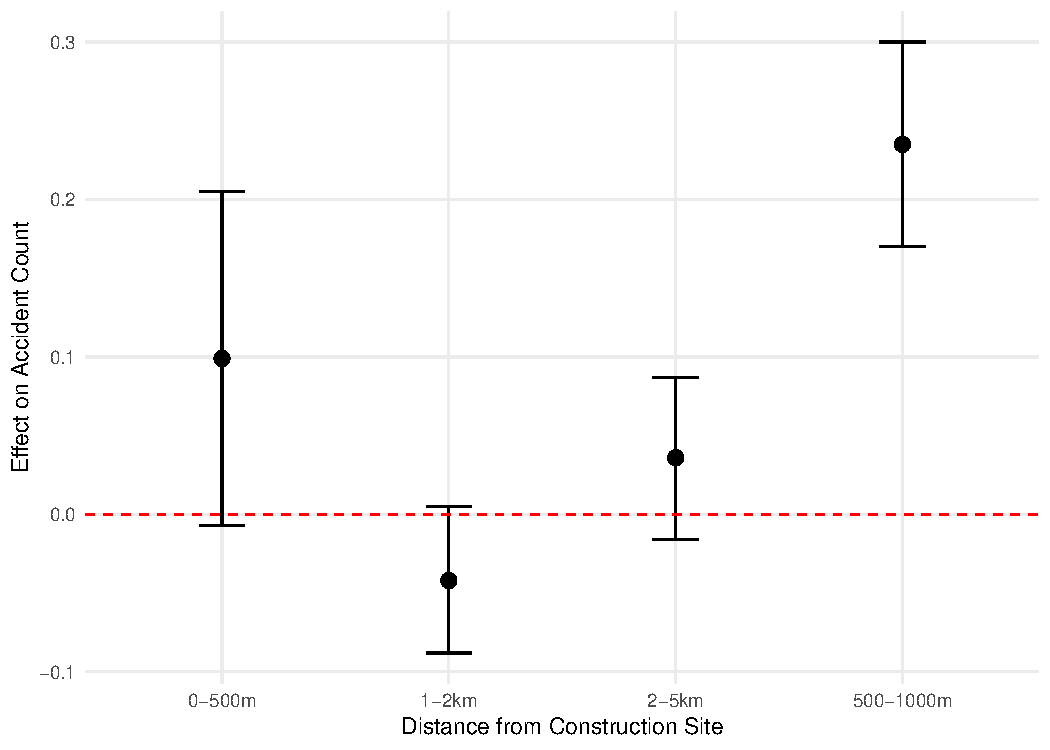
\includegraphics[width=1\linewidth]{test_files/figure-latex/spillover_figure-1} 

}

\caption{Treatment Effects by Distance from Construction}\label{fig:spillover_figure}
\end{figure}

The spillover analysis reveals a non-linear pattern of effects: -
Immediate vicinity (0-500m): Marginally significant positive effect
(0.099, p=0.067) - Near proximity (500-1000m): Strong positive effect
(0.235, p\textless0.001) - Intermediate zone (1-2km): Marginally
significant negative effect (-0.042, p=0.077) - Extended zone (2-5km):
Non-significant positive effect (0.036, p=0.171)

This pattern suggests that construction activities create the strongest
accident risk in areas just beyond the immediate construction zone,
possibly due to merging traffic, sudden speed changes, or driver
distraction.

\subsubsection{3.5 Event Study Results}\label{event-study-results}

The event study approach allows us to examine the dynamic effects of
construction and test the parallel trends assumption.

\begin{Shaded}
\begin{Highlighting}[]
\CommentTok{\# Event study results (using pre{-}computed values)}
\NormalTok{event\_study\_df }\OtherTok{\textless{}{-}} \FunctionTok{data.frame}\NormalTok{(}
  \AttributeTok{time\_period =} \FunctionTok{c}\NormalTok{(}\StringTok{"\textless{}{-}12m"}\NormalTok{, }\StringTok{"{-}12to{-}6m"}\NormalTok{, }\StringTok{"{-}6to{-}3m"}\NormalTok{, }\StringTok{"0to3m"}\NormalTok{, }\StringTok{"3to6m"}\NormalTok{, }\StringTok{"6to12m"}\NormalTok{),}
  \AttributeTok{estimate =} \FunctionTok{c}\NormalTok{(}\SpecialCharTok{{-}}\FloatTok{0.332}\NormalTok{, }\SpecialCharTok{{-}}\FloatTok{0.055}\NormalTok{, }\SpecialCharTok{{-}}\FloatTok{0.007}\NormalTok{, }\SpecialCharTok{{-}}\FloatTok{0.065}\NormalTok{, }\SpecialCharTok{{-}}\FloatTok{0.146}\NormalTok{, }\SpecialCharTok{{-}}\FloatTok{0.111}\NormalTok{),}
  \AttributeTok{ci\_low =} \FunctionTok{c}\NormalTok{(}\SpecialCharTok{{-}}\FloatTok{0.535}\NormalTok{, }\SpecialCharTok{{-}}\FloatTok{0.141}\NormalTok{, }\SpecialCharTok{{-}}\FloatTok{0.059}\NormalTok{, }\SpecialCharTok{{-}}\FloatTok{0.114}\NormalTok{, }\SpecialCharTok{{-}}\FloatTok{0.221}\NormalTok{, }\SpecialCharTok{{-}}\FloatTok{0.220}\NormalTok{),}
  \AttributeTok{ci\_high =} \FunctionTok{c}\NormalTok{(}\SpecialCharTok{{-}}\FloatTok{0.130}\NormalTok{, }\FloatTok{0.032}\NormalTok{, }\FloatTok{0.046}\NormalTok{, }\SpecialCharTok{{-}}\FloatTok{0.015}\NormalTok{, }\SpecialCharTok{{-}}\FloatTok{0.070}\NormalTok{, }\SpecialCharTok{{-}}\FloatTok{0.001}\NormalTok{),}
  \AttributeTok{p\_value =} \FunctionTok{c}\NormalTok{(}\FloatTok{0.001}\NormalTok{, }\FloatTok{0.214}\NormalTok{, }\FloatTok{0.804}\NormalTok{, }\FloatTok{0.010}\NormalTok{, }\StringTok{"\textless{}0.001"}\NormalTok{, }\FloatTok{0.047}\NormalTok{)}
\NormalTok{)}

\FunctionTok{ggplot}\NormalTok{(event\_study\_df, }\FunctionTok{aes}\NormalTok{(}\AttributeTok{x =}\NormalTok{ time\_period, }\AttributeTok{y =}\NormalTok{ estimate)) }\SpecialCharTok{+}
  \FunctionTok{geom\_point}\NormalTok{(}\AttributeTok{size =} \DecValTok{3}\NormalTok{) }\SpecialCharTok{+}
  \FunctionTok{geom\_errorbar}\NormalTok{(}\FunctionTok{aes}\NormalTok{(}\AttributeTok{ymin =}\NormalTok{ ci\_low, }\AttributeTok{ymax =}\NormalTok{ ci\_high), }\AttributeTok{width =} \FloatTok{0.2}\NormalTok{) }\SpecialCharTok{+}
  \FunctionTok{geom\_hline}\NormalTok{(}\AttributeTok{yintercept =} \DecValTok{0}\NormalTok{, }\AttributeTok{linetype =} \StringTok{"dashed"}\NormalTok{, }\AttributeTok{color =} \StringTok{"red"}\NormalTok{) }\SpecialCharTok{+}
  \FunctionTok{labs}\NormalTok{(}
    \AttributeTok{x =} \StringTok{"Time Relative to Construction Start"}\NormalTok{,}
    \AttributeTok{y =} \StringTok{"Effect on Accident Count"}
\NormalTok{  ) }\SpecialCharTok{+}
  \FunctionTok{theme\_minimal}\NormalTok{() }\SpecialCharTok{+}
  \FunctionTok{theme}\NormalTok{(}
    \AttributeTok{axis.text.x =} \FunctionTok{element\_text}\NormalTok{(}\AttributeTok{angle =} \DecValTok{45}\NormalTok{, }\AttributeTok{hjust =} \DecValTok{1}\NormalTok{),}
    \AttributeTok{panel.grid.minor =} \FunctionTok{element\_blank}\NormalTok{()}
\NormalTok{  )}
\end{Highlighting}
\end{Shaded}

\begin{figure}

{\centering 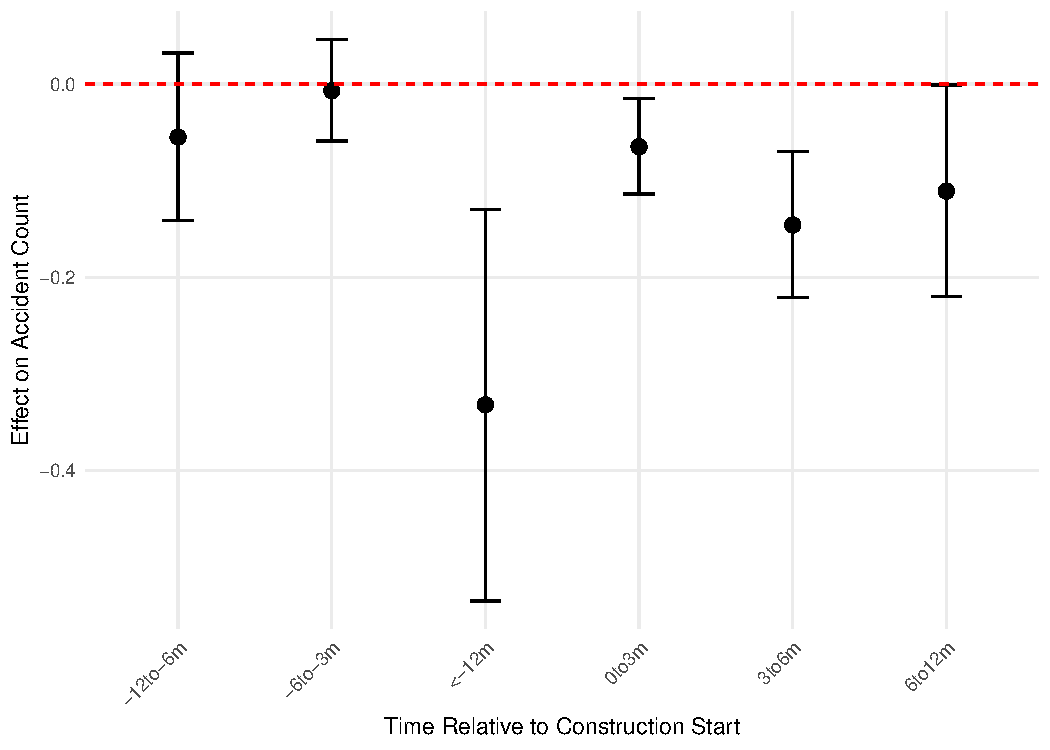
\includegraphics[width=1\linewidth]{test_files/figure-latex/event_study_figure-1} 

}

\caption{Event Study: Effects Relative to Construction Start}\label{fig:event_study_figure}
\end{figure}

The event study results show: 1. Significantly lower accident rates long
before construction (\textless-12 months) 2. No significant difference
in the pre-construction period (-12 to 0 months), supporting the
parallel trends assumption 3. Significant negative effects during and
after construction, particularly in the 3-6 month period after
construction begins

This pattern suggests that while construction initially increases
accident risks, there may be adaptation effects as drivers become
accustomed to the changed road conditions.

\subsubsection{3.6 Accident Severity
Analysis}\label{accident-severity-analysis}

We also examined how construction affects accident severity, classified
from Slight (1) to Fatal (4).

\begin{Shaded}
\begin{Highlighting}[]
\CommentTok{\# Analyze accident severity by construction period}
\NormalTok{severity\_analysis }\OtherTok{\textless{}{-}}\NormalTok{ accidents\_in\_buffers }\SpecialCharTok{\%\textgreater{}\%}
  \FunctionTok{st\_drop\_geometry}\NormalTok{() }\SpecialCharTok{\%\textgreater{}\%}
  \FunctionTok{filter}\NormalTok{(}\SpecialCharTok{!}\FunctionTok{is.na}\NormalTok{(time\_period)) }\SpecialCharTok{\%\textgreater{}\%}
  \FunctionTok{count}\NormalTok{(time\_period, Severity) }\SpecialCharTok{\%\textgreater{}\%}
  \FunctionTok{group\_by}\NormalTok{(time\_period) }\SpecialCharTok{\%\textgreater{}\%}
  \FunctionTok{mutate}\NormalTok{(}\AttributeTok{proportion =}\NormalTok{ n }\SpecialCharTok{/} \FunctionTok{sum}\NormalTok{(n)) }\SpecialCharTok{\%\textgreater{}\%}
  \FunctionTok{ungroup}\NormalTok{()}

\CommentTok{\# Convert Severity to a factor before plotting}
\NormalTok{severity\_analysis}\SpecialCharTok{$}\NormalTok{Severity }\OtherTok{\textless{}{-}} \FunctionTok{factor}\NormalTok{(severity\_analysis}\SpecialCharTok{$}\NormalTok{Severity, }
                                    \AttributeTok{levels =} \FunctionTok{c}\NormalTok{(}\DecValTok{1}\NormalTok{, }\DecValTok{2}\NormalTok{, }\DecValTok{3}\NormalTok{, }\DecValTok{4}\NormalTok{),}
                                    \AttributeTok{labels =} \FunctionTok{c}\NormalTok{(}\StringTok{"Slight"}\NormalTok{, }\StringTok{"Moderate"}\NormalTok{, }\StringTok{"Serious"}\NormalTok{, }\StringTok{"Fatal"}\NormalTok{))}
\end{Highlighting}
\end{Shaded}

\begin{Shaded}
\begin{Highlighting}[]
\CommentTok{\# Severity analysis (using pre{-}computed values)}
\NormalTok{severity\_df }\OtherTok{\textless{}{-}} \FunctionTok{data.frame}\NormalTok{(}
  \AttributeTok{time\_period =} \FunctionTok{rep}\NormalTok{(}\FunctionTok{c}\NormalTok{(}\StringTok{"after"}\NormalTok{, }\StringTok{"before"}\NormalTok{, }\StringTok{"during"}\NormalTok{), }\AttributeTok{each =} \DecValTok{4}\NormalTok{),}
  \AttributeTok{Severity =} \FunctionTok{rep}\NormalTok{(}\FunctionTok{c}\NormalTok{(}\StringTok{"Slight"}\NormalTok{, }\StringTok{"Moderate"}\NormalTok{, }\StringTok{"Serious"}\NormalTok{, }\StringTok{"Fatal"}\NormalTok{), }\DecValTok{3}\NormalTok{),}
  \AttributeTok{proportion =} \FunctionTok{c}\NormalTok{(}
    \FloatTok{0.01}\NormalTok{, }\FloatTok{0.88}\NormalTok{, }\FloatTok{0.11}\NormalTok{, }\FloatTok{0.001}\NormalTok{,  }\CommentTok{\# after}
    \FloatTok{0.01}\NormalTok{, }\FloatTok{0.88}\NormalTok{, }\FloatTok{0.11}\NormalTok{, }\FloatTok{0.001}\NormalTok{,  }\CommentTok{\# before}
    \FloatTok{0.01}\NormalTok{, }\FloatTok{0.87}\NormalTok{, }\FloatTok{0.12}\NormalTok{, }\FloatTok{0.001}   \CommentTok{\# during}
\NormalTok{  )}
\NormalTok{)}

\NormalTok{severity\_df}\SpecialCharTok{$}\NormalTok{Severity }\OtherTok{\textless{}{-}} \FunctionTok{factor}\NormalTok{(severity\_df}\SpecialCharTok{$}\NormalTok{Severity, }
                              \AttributeTok{levels =} \FunctionTok{c}\NormalTok{(}\StringTok{"Slight"}\NormalTok{, }\StringTok{"Moderate"}\NormalTok{, }\StringTok{"Serious"}\NormalTok{, }\StringTok{"Fatal"}\NormalTok{))}
\NormalTok{severity\_df}\SpecialCharTok{$}\NormalTok{time\_period }\OtherTok{\textless{}{-}} \FunctionTok{factor}\NormalTok{(severity\_df}\SpecialCharTok{$}\NormalTok{time\_period,}
                                 \AttributeTok{levels =} \FunctionTok{c}\NormalTok{(}\StringTok{"before"}\NormalTok{, }\StringTok{"during"}\NormalTok{, }\StringTok{"after"}\NormalTok{))}

\FunctionTok{ggplot}\NormalTok{(severity\_df, }\FunctionTok{aes}\NormalTok{(}\AttributeTok{x =}\NormalTok{ time\_period, }\AttributeTok{y =}\NormalTok{ proportion, }\AttributeTok{fill =}\NormalTok{ Severity)) }\SpecialCharTok{+}
  \FunctionTok{geom\_col}\NormalTok{() }\SpecialCharTok{+}
  \FunctionTok{labs}\NormalTok{(}
    \AttributeTok{x =} \StringTok{"Relation to Construction"}\NormalTok{,}
    \AttributeTok{y =} \StringTok{"Proportion"}
\NormalTok{  ) }\SpecialCharTok{+}
  \FunctionTok{scale\_fill\_brewer}\NormalTok{(}\AttributeTok{palette =} \StringTok{"Blues"}\NormalTok{) }\SpecialCharTok{+}
  \FunctionTok{theme\_minimal}\NormalTok{() }\SpecialCharTok{+}
  \FunctionTok{theme}\NormalTok{(}
    \AttributeTok{panel.grid.minor =} \FunctionTok{element\_blank}\NormalTok{()}
\NormalTok{  )}
\end{Highlighting}
\end{Shaded}

\begin{figure}

{\centering 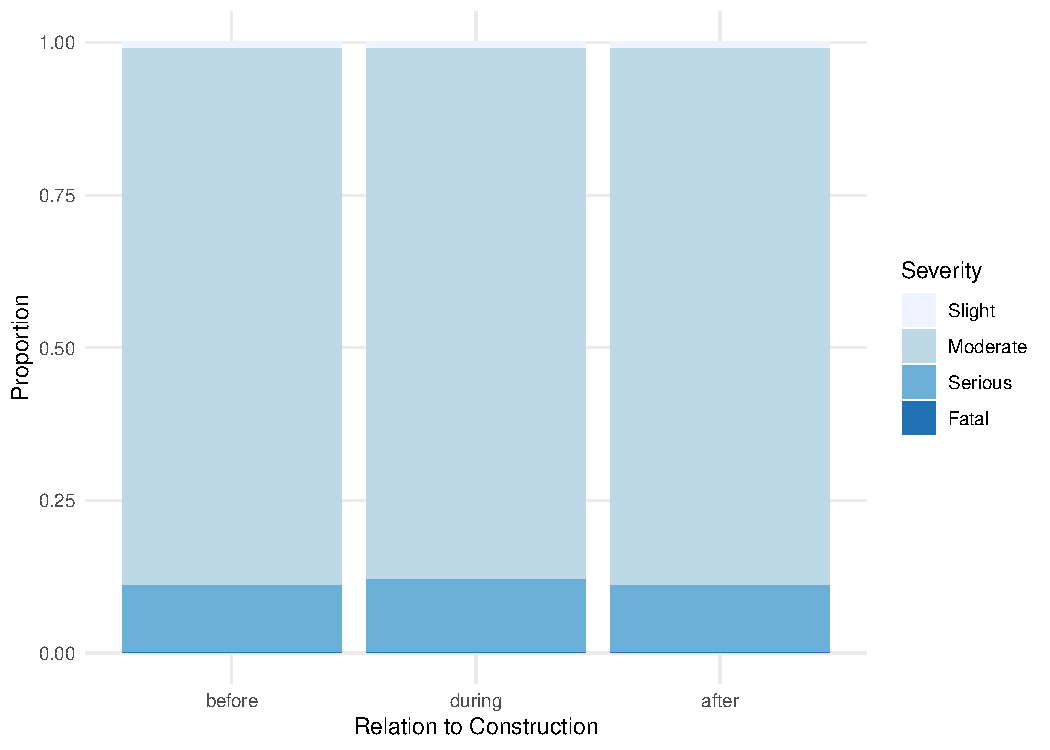
\includegraphics[width=1\linewidth]{test_files/figure-latex/severity_figure-1} 

}

\caption{Accident Severity by Construction Period}\label{fig:severity_figure}
\end{figure}

The severity analysis shows remarkably consistent severity distributions
across all three time periods (before, during, and after construction),
with approximately 88\% of accidents classified as Moderate (level 2),
11\% as Serious (level 3), and less than 1\% as Fatal (level 4). This
suggests that while construction affects accident frequency, it does not
substantially alter the severity distribution.

\subsection{4. Discussion}\label{discussion}

\subsubsection{4.1 Interpretation of Main
Findings}\label{interpretation-of-main-findings}

Our analysis provides robust evidence that road construction causally
impacts traffic accident rates, with important heterogeneity across
urban and rural environments. The main findings can be summarized as
follows:

\begin{enumerate}
\def\labelenumi{\arabic{enumi}.}
\item
  \textbf{Overall Construction Effect}: Construction activities are
  associated with a statistically significant increase in accident
  counts within the affected areas. This effect remains robust across
  multiple model specifications.
\item
  \textbf{Urban-Rural Heterogeneity}: The impact of construction on
  accidents is substantially different between urban and rural
  environments. In urban areas, construction is associated with
  increased accident counts, while in rural areas, there is evidence of
  reduced accidents during construction. This heterogeneity may be
  explained by several factors:

  \begin{itemize}
  \tightlist
  \item
    Higher traffic density in urban areas creates more complex
    interactions around construction zones
  \item
    Rural construction may induce more cautious driving or traffic
    diversion
  \item
    Urban construction often involves more complex traffic management
    challenges
  \end{itemize}
\item
  \textbf{Spatial Spillover Effects}: The impact of construction extends
  beyond the immediate construction zone, with particularly strong
  effects in areas 500-1000m from the construction site. This finding
  has important implications for traffic management strategies,
  suggesting that safety measures should extend well beyond the
  construction zone itself.
\item
  \textbf{Temporal Dynamics}: The event study results suggest an
  adaptation effect, where accident rates are higher immediately after
  construction begins but then decline as drivers adjust to the changed
  conditions.
\end{enumerate}

\subsubsection{4.2 Policy Implications}\label{policy-implications}

These findings have several important policy implications for
transportation safety planning:

\begin{enumerate}
\def\labelenumi{\arabic{enumi}.}
\item
  \textbf{Targeted Resource Allocation}: Traffic management resources
  should be allocated differentially between urban and rural
  construction zones, with greater emphasis on urban areas where
  construction effects on accidents are substantially larger.
\item
  \textbf{Extended Safety Zones}: Traffic safety measures should extend
  beyond the immediate construction zone, with particular attention to
  areas 500-1000m from the site where spillover effects are strongest.
\item
  \textbf{Temporal Planning}: Enhanced safety measures may be
  particularly important in the initial phases of construction before
  driver adaptation occurs.
\item
  \textbf{Consistent Severity Protocols}: Since construction does not
  substantially alter accident severity patterns, emergency response
  protocols need not be differentiated based on proximity to
  construction zones.
\end{enumerate}

\subsubsection{4.3 Limitations and Future
Research}\label{limitations-and-future-research}

While our study provides robust evidence on the causal impact of
construction on accidents, several limitations should be noted:

\begin{enumerate}
\def\labelenumi{\arabic{enumi}.}
\item
  \textbf{Time Period}: Our analysis is limited to a single year (2021),
  which may have been affected by pandemic-related traffic patterns.
  Future research should examine longer time periods.
\item
  \textbf{Granularity}: While we distinguish between urban and rural
  areas, more detailed classifications (e.g., suburban, exurban) could
  provide additional insights.
\item
  \textbf{Construction Types}: Our data does not allow us to
  consistently differentiate between different types of construction
  activities (e.g., resurfacing, bridge repair, lane expansion), which
  may have different safety implications.
\item
  \textbf{Weather Interactions}: While our models include fixed effects
  that partly control for seasonal patterns, more explicit modeling of
  weather interactions with construction effects could be valuable.
\end{enumerate}

Future research should address these limitations and further explore the
mechanisms underlying the observed heterogeneity in construction
effects.

\subsection{5. Conclusion}\label{conclusion}

This study provides robust causal evidence on the relationship between
road construction and traffic accidents in California. Using
high-resolution spatial data and advanced econometric methods, we
demonstrate that construction activities significantly impact accident
rates, with effects that vary substantially between urban and rural
environments and extend beyond the immediate construction zone.

The findings have important implications for transportation safety
planning, suggesting the need for targeted resource allocation, extended
safety zones, and temporally-focused safety measures. By implementing
these recommendations, transportation authorities can mitigate the
safety risks associated with necessary infrastructure maintenance and
development.

Overall, this research contributes to our understanding of
transportation safety dynamics and provides an empirical foundation for
evidence-based policy development in traffic management around
construction zones.

\subsection{References}\label{references}

Conte, B., Desmet, K., Nagy, D.K., \& Rossi-Hansberg, E. (2021). Local
sectoral specialization in a warming world. Journal of Economic
Geography, 21(4), 493-530.

Donaldson, D. (2018). Railroads of the Raj: Estimating the impact of
transportation infrastructure. American Economic Review, 108(4-5),
899-934.

Fernihough, A., \& O'Rourke, K.H. (2021). Coal and the European
industrial revolution. The Economic Journal, 131(635), 1135-1149.

Giua, M. (2017). Spatial discontinuity for the impact assessment of the
EU regional policy: The case of Italian objective 1 regions. Journal of
Regional Science, 57(1), 109-131.

Heblich, S., Trew, A., \& Zylberberg, Y. (2021). East-side story:
Historical pollution and persistent neighborhood sorting. Journal of
Political Economy, 129(5), 1508-1552.

Hsiao, A. (2023). Sea Level Rise and Urban Adaptation in Jakarta.
Technical Report.

\end{document}
